\documentclass[aps,reprint]{revtex4-1}
% Engine-specific settings
% Detect pdftex/xetex/luatex, and load appropriate font packages.
% This is inspired by the approach in the iftex package.
% pdftex:
\ifx\pdfmatch\undefined
\else
    \usepackage[T1]{fontenc}
    \usepackage[utf8]{inputenc}
\fi
% xetex:
\ifx\XeTeXinterchartoks\undefined
\else
    \usepackage{fontspec}
    \defaultfontfeatures{Ligatures=TeX}
\fi
% luatex:
\ifx\directlua\undefined
\else
    \usepackage{fontspec}
\fi
% End engine-specific settings
\usepackage[english]{babel}
\usepackage{csquotes}
% \usepackage[backend=biber, sortcites]{biblatex}
\usepackage{url}
\usepackage{textcomp}
\usepackage[usenames,dvipsnames,svgnames, table]{xcolor}
\usepackage[font={scriptsize}]{caption}
\usepackage{amsmath} \usepackage{amsthm} \usepackage{amsfonts}
\usepackage{amssymb}
\usepackage{enumerate}
\usepackage{tikz} \usepackage{float}
\usepackage[procnames]{listings}
\usepackage{pstool} \usepackage{pgfplots}
\usepackage{wrapfig} \usepackage{graphicx} \usepackage{epstopdf}
\usepackage{afterpage}
\usepackage{physics}
\usepackage{multirow}
\usepackage{gensymb}
\usepackage{algorithm}
\usepackage{microtype}
\usepackage[noend]{algpseudocode}
\usepackage{xcolor,colortbl}
\usepackage{microtype}
\usepackage{geometry}
\usepackage{hyperref}
\usepackage{graphicx}
\usepackage{caption}
\usepackage{subcaption}
\usepackage{lipsum}
% \usepackage{pythontex}
% \usepackage{authblk}
\usepackage{nth}
\usepackage{siunitx}
% \usepackage[toc,page]{appendix}
\floatstyle{plaintop}
\restylefloat{table}

% Custom commands
\newcommand{\unit}[1]{\:\mathrm{#1}}
\newcommand{\noref}[1]{\hyperref[#1]{\ref*{#1}}}
\newcommand{\nonref}[1]{\hyperref[]{\ref*{#1}}}
\newcommand\blankpage{%
  \null
  \thispagestyle{empty}%
  \addtocounter{page}{-1}%
  \newpage}

% Default fixed font does not support bold face
\DeclareFixedFont{\ttb}{T1}{txtt}{bx}{n}{7} % for bold
\DeclareFixedFont{\ttm}{T1}{txtt}{m}{n}{7}  % for normal

\newcommand\numberthis{\addtocounter{equation}{1}\tag{\theequation}}
\DeclareCaptionFont{white}{\color{white}}
\DeclareCaptionFormat{listing}{\colorbox{gray}{\parbox{\columnwidth}{#1#2#3}}}
\pgfplotsset{compat=1.14} %TODO: Setting this removed several error messages, should it be here!?


% Biber for references
% \bibliographystyle{aipauth4-1}

\begin{document}
\sisetup{detect-all}
\title{Simulation of the solar system with numerical methods}
\author{Erlend Lima}
\author{Frederik J. Mellbye}
\affiliation{University of Oslo, Oslo, Norway \\ Source code available at: \url{https://github.com/Caronthir/FYS3150/tree/master/Project3}}
\date{\today}

\begin{abstract}
Two numerical algorithms are used to solve systems of coupled ODE's representing
the\(n\)-body problem of the solar system, namely Forward Euler and Velocity-Verlet. With
only two additional floating point operations per
iteration of the algorithm, the Verlet method is shown to completely outperform
the Euler scheme in terms of numerical accuracy and stability,
with a small cost in execution speed. By investigating the solutions for
different step sizes, $10^5$ time steps per year resulted in
solutions with an acceptable compromise between numerical precision and speed.
The perihelion precession of Mercury resulting from a relativistic correction
was also reproduced to be \(42.39''\) where the theoretical value is \(43''\).
\end{abstract}
\maketitle
\tableofcontents
\makeatletter
\let\toc@pre\relax
\let\toc@post\relax
\makeatother

\newpage

\section{Introduction}
\label{sec:introduction}
The \(n\)-body problem consists of predicting the individual motion of a group of objects
interacting with every other object through some force. This might be celestial
bodies dancing together through gravity, or molecules jiggling from
electromagnetism. It is trivial to find an analytical solution for a system of
two bodies, but for three or more bodies, an analytical solution does not exist
spare a few special cases. Instead, one have to resort to approximations.

In this paper, the equations of motion are written as a coupled set of first-order linear equations, and
the classic forward Euler and Velocity Verlet algorithms are employed to simulate the solar system,
and their accuracies, conservation properties and computation times are compared. The theoretical
model for the forces in our solar system (Newtonian gravity) is shown, and the numerical implementations
are used to solve the time development of the planets in the solar system. Several analytical results
are reproduced by the program, such as conservation of energy and angular momentum, escape velocities
and the perihelion precession of Mercury.
\section{Theory}
\label{sec:theory}
\subsection{Newtonian gravity}
Planetary motion is only governed by gravity. Newton's law of gravitation
states that any two objects in the universe attract each other by a force given
by
\begin{align}
  F_G = \frac{G m_1 m_2}{r^2}
\end{align}
where $m_1$ and $m_2$ are the masses of the objects, $G$ is the
gravitational constant and $r$ is the distance between the objects. In the
case examined in this paper, it is assumed that the solar mass is much larger
than the planet masses ($M_\odot \gg M_\text{planet}$), and the solar
movement is therefore ignored unless otherwise specified.
For a planet orbiting the sun, the
planet position as a function of time is described by Newton's second law:
\begin{align*}
  \dv[2]{\mathbf{x}}{t} = \frac{\mathbf{F}_G}{M}
\end{align*}
where $M$ is the planet mass. This is equivalent to one ODE (ordinary differential
equation) for each direction component, i.e.\@ three coupled equations in the
three-dimensional case.

For the numerical methods the above second order vector ODE is more convenient to
work with when written as a set of two coupled first order equations. These
are given by
\begin{align}
  \begin{split}
  \label{eq:coupledequations}
  \dv{x}{t} &= v(x,t) \\
  \dv{v}{t} &= \frac{F(x,t)}{M} = a(x,t)
  \end{split}
\end{align}
These equations are solved for three dimensions. Note that the gravitational force,
and hence the acceleration, depends on the distance between the celestial bodies.
This results in six coupled, first-order, linear differential equations.

\subsection{Numerical algorithms}
\label{sec:numalgos}
The algorithms used are both based on Taylor expansions. The forward Euler
scheme approximates position and velocity to first order, while the Verlet
method combines a second order approximation with the fact that the acceleration
is only position dependent.

For both methods, the time is discretized to $N$ integration points so that
\begin{align*}
  t \rightarrow t_i = t_0 + i \Delta{t}
\end{align*}
where $\Delta{t} = \frac{t_\text{f} - t_0}{N}$ is the time step and $i = 0, 1, \hdots, N$.
From this a discretization of position follows, i.e.
\begin{align*}
  x(t) = x(t_i) \rightarrow x_i
\end{align*}
and similarly for velocity and acceleration so that $v(t_i) \rightarrow v_i$ and
$a(t_i) \rightarrow a_i$.

\subsubsection{Forward Euler}
The Euler method (forward Euler) is the most basic numerical method to solve
ODEs. This widely known algorithm applied to~\ref{eq:coupledequations} is given by
\begin{align*}
  \begin{split}
  v_{i+1} = v_{i} + a_{i}\Delta{t} \\
  x_{i+1} = x_{i} + v_{i}\Delta{t}
\end{split}
\end{align*}
These equations are derived by simply Taylor expanding the position and velocity
and omitting the error terms.
\subsubsection{Velocity Verlet}
The velocity Verlet method is based on Taylor-expanding the position and velocity
to second order, and specialized for cases where the acceleration is only
dependent on position. The algorithm (see appendix~\ref{sec:velocityverlet} for details)
applied to the problem examined in this paper is given by the following equations:
\begin{align}
  \begin{split}
    x_{i+1} &= x_i + v_i + \frac{\Delta{t}^2}{2} a_i \\
    v_{i+1} &= v_i + \frac{\Delta{t}}{2}(a_{i+1} + a_{i})
  \end{split}
\end{align}
Note that this algorithm assumes $a_{i+1}$ is only dependent on position $x_{i+1}$
and not velocity $v_{i+1}$. This is because the acceleration in the next step
is required to calculate the velocity in the next step. Because $a_{i+1} = a(x_{i+1})$,
the position in the next step is computed prior to the velocity. This algorithm
therefore is suited to solve for planetary motion, because gravity is only
position dependent and the only force that acts within the system.
\subsubsection{Comparison of number of floating point operations}
Before the solver is implemented and the timings are compared, it is interesting
to compare the number of FLOPS (floating point operations) per iteration of the
algorithms. Both lines of the Euler simulation requires two FLOPS (one
multiplication and one addition), which sums to four operations per iteration.
With the Verlet method, the quantity $\Delta{t}^2 / 2$ can be precomputed and
$a_{i}$ only needs to be computed once per iteration and saved for the next.
The Verlet method therefore requires six FLOPS per iteration. The calculation
of the accelerations has not been considered, but it is easy to conclude that
as more planets are added to the system a smaller relative difference in timings
should be observed between the two forwarding algorithms.
\subsection{Initial conditions}
To find a unique solution to the set of coupled equations a set of initial conditions needs
to be specified. For the set of three coupled second order equations solved in this project,
initial positions and velocities are required for each spatial dimension. That is,
\begin{align*}
 \mathbf{x_0}(t = 0) \text{ and } \mathbf{v_0}(t = 0)
\end{align*}
are required for the sun and all planets and moons that are included in the simulation.

\subsection{Conservation laws for the system}
Because no external forces act on the system, total energy and angular momentum should
be conserved over time. Expressions for these quantities are shown separately.
\subsubsection{Energy}
The total energy of the system should be conserved. The kinetic energy of an object with
mass $m$ and velocity $v$ is given by
\begin{align*}
 E_k = \frac{1}{2}m v^2
\end{align*}
The expression for the gravitational potential energy of a massive object can be found by
integrating the gravitational force from the distance between the objects to some reference
distance, which is set to $r = \infty$ (i.e. using the definition of potential energy and the law
of gravitation). This yields
\begin{align*}
  \label{eq:potentialenergy}
 E_p = -\int_\infty^r F_G\: \text{d} r = -\frac{GmM}{r}
\end{align*}
as the potential energy of an object (mass $m$) with respect to some object (mass $M$),
separated by a distance $r$.
\subsubsection{Angular momentum}
The total angular momentum of the system should also be conserved. The orbital
angular momentum of an object is given as
\begin{align}
  \mathbf{L} = \mathbf{r} \times \mathbf{p}
\end{align}
where $\mathbf{p} = m \mathbf{v}$ is the momentum of the object and $\mathbf{r}$
is the position of the object with respect to the system center of mass (COM).
\subsection{Escape velocity}
The escape velocity is the minimum speed needed for an object to escape from the
gravitational influence of an object with mass. The expression for the escape
velocity of an object in the gravitational field of some other object with mass
$M_\odot$ at a distance $r$ is given by
\begin{align}
  \label{eq:escapevelocity}
  v_e = |\mathbf{v_e}| = \sqrt{\frac{2GM_\odot}{r}}
\end{align}
See appendix~\ref{sec:escapevelocityderivation} for a complete derivation of this expression.

\subsection{Perihelion precession of Mercury}
In Newtonian physics, any object that orbits a massive star or planet will have an elliptical orbit with
the spherical mass approximately at focus. In the solar system, the closest point to the Sun of an orbit is called
the perihelion. Multiple effects in the solar system cause the elliptical orbits
to rotate, in the sense that the perihelion
precesses around the sun. The most significant effect comes from the gravitational forces from the other bodies in
the solar system. The Newtonian based-explanations were insufficient in
predicting the perihelion precession of Mercury, but
this was corrected when Einstein showed that results from general relativity closely agrees with the observed
perihelion precession. To correct for general relativity spacetime shift, the gravitational force can be modified to
\begin{align}
\label{eq:mercuryprecession}
\mathbf{F_G} = \frac{G M_\odot M_\text{Mercury}}{r^2}\left[1 + \frac{3l^2}{r^2c^2} \right] \hat{\mathbf{r}}
\end{align}
where $l = |\mathbf{l}|$ is the norm of the angular momentum per mass of Mercury, $c$ is the speed of light and
$\mathbf{r}$ is the relative position of Mercury with respect to the Sun. See \cite{project3}
for a more complete description.
\section{Method}
\label{sec:method}
\subsection{Choice of units}
For the Solar System it is convenient to use units that scale lengths, time and
masses to orders of magnitude that are easier to work with. The distances are
therefore in astronomical units (AU), which is defined to roughly the mean
distance between the Earth and the Sun. By the same token, time is measured in
years (yr) and masses are in solar masses $M_\odot$.

Examining Newton's law for Earth in the Earth-Sun system under the assumption
that the orbit is circular shows that
\begin{align*}
  \frac{GmM_\odot}{r^2} = m \frac{v^2}{r}
\end{align*}
where $m$ is Earth's mass and $r$ is the distance between the objects. In the
units chosen, $r = 1$ AU and the orbital velocity is given by the orbital distance
travelled per year $v = 2\pi \text{AU}/1 \text{yr}$. Then the gravitational
constant is given by
\begin{align}
  G = 4\pi^2 \text{AU}^3 \text{yr}^{-2} M_\odot^{-1}
\end{align}
\subsection{Initial values}
The initial values of the solar system bodies are fetched from the NASA HORIZONS
Web-Interface, see \cite{nasa}. This process was automated with the Python script
\texttt{getnasa.py} (See git repository).
\subsection{Calculation of conserved properties}
\subsubsection{Total energy}
The total energy and it's distribution among total potential and kinetic energy
is monitored for each simulation. The total energy of the solar system at a given time step is
calculated by summing the total energy of each planet at each time step.
At a given time step $t_i$, the kinetic energy of a given planet with mass $m$
and discretized velocity $v_i$ is simply given by
\begin{align}
  K_i = \frac{1}{2} m v_i^2
\end{align}
The potential energy of a planet is given by~\eqref{eq:potentialenergy}.
This needs to be summed for each distance $r$ between the respective planets. To
avoid double-counting the potential energies, the potential energy is calculated
as
\begin{align}
  U_{i, \text{tot}} = \sum_j \sum_{i > j} - \frac{G M_j M_i}{|\mathbf{x}_i - \mathbf{x}_j|}
\end{align}
where $M_i$ is the mass and $\mathbf{x}_i$ the position of planet number $i$
(the planets are indexed). The total energy is then
\begin{align}
  E_{i,\text{tot}} = K_i + U_i
\end{align}
\subsubsection{Angular momentum}
The total angular momentum is calculated by summing the angular momenta of
every object in the system. The calculation can simply be written as
\begin{align}
  \mathbf{L}_i = \sum_j \mathbf{r}_{j,i} \times \mathbf{p}_{j,i}
\end{align}
where $j$ indicates the planet index, $i$ is the time step index and $\mathbf{r}$ is the
position relative to the center of mass. The center of mass of the system
is calculated with
\begin{align}
  \mathbf{R}_\text{COM} = \frac{1}{M_\text{tot}} \sum_j M_j \mathbf{r}_j
\end{align}
\subsubsection{Relative quantities}
In the analysis, because of the unusual units used, it is more intuitive to
consider the relative energy (the energy divided by the initial energy). At time step $i$
this is given by
\begin{align}
  E_i = \frac{E_{i,\text{tot}}}{E_{0,\text{tot}}}
\end{align}
The relative energy is referred to as the energy $E$ in the results and
discussion. The total angular momentum is scaled similarly.

\subsection{Bisection method to find escape velocities numerically}
Applying~\eqref{eq:escapevelocity} to the Earth-Sun system, the Earth requires an initial velocity of
$v = 2 \pi \sqrt{2}$ AU/yr to escape the solar system.

A bisection inspired method was developed to find this value numerically. For the
full algorithm see \texttt{findescapevelocity.py} in the Git repository. A challenge
with this method was to determine the amount of years of simulation required to
determine if the planet has escaped or not. As the initial velocity of the Earth
approaches the escape velocity, the Earth will take longer and longer to change
direction and fall back towards the sun. Taking this to the limit, the Earth will
simply come to a halt ``at the end of'' the solar system. Finding the escape
velocity of the earth is therefore infeasible as the simulation would have to
run for an infinite amount of time. Instead, the simulation period was increased
steadily after the bisection method converged, showing how the escape velocity
converged to \(2\pi\sqrt{2}\) as time increased.

The force of gravity was then modified by changing the exponent for the radius
in the force expression, i.e. a modification of the type
\begin{equation}
  \label{eq:duckling}
  \tilde{F}_G = \frac{G m_1 m_2}{r^\beta}
\end{equation}
where $\beta \in [2,3]$ are tested. Notice that $\beta = 2$ results in the correct
Newtonian expression. The escape velocity was then computed with the method
described above for multiple $\beta$.

\subsection{Models}
In this project, four separate situations are tested. This makes it possible to test the versatility of the
algorithms in different circumstances and to investigate multiple special situations.
\subsubsection{Earth-Sun system - Comparison of Forward Euler and Velocity-Verlet}
\label{seq:earthsunmethod}
For the simple case of the Earth-Sun system, the positions of the Sun and Earth are
forwarded for a year with both algorithms. The Sun is placed at the origin with
no initial velocity, and for simplicity Earth is given an initial position 1 AU
away from the Sun in the x-direction. It is given an initial velocity $v = 2\pi$ AU/yr
in the y-direction, which analytically should lead to a perfect circular motion
if the Sun is kept stationary. The simulation is done with $N = 1000$ time steps.
The total energy in the system over time is shown in a plot, and used for
comparing the algorithms.

This simulation was then ran for multiple numbers of steps per year, and for
each simulation the energy and total runtime in C++ was fetched.
\subsubsection{Three-body problem}
The Earth-Sun system is expanded to include the most massive planet in the Solar System, Jupiter.
An ideal number of time steps per year is found by trial and error. In this and the remaining models, the Velocity
Verlet algorithm is used because of the far superior accurary compared to the
Euler scheme. The impact of the inclusion of Jupiter on the Earth orbit is investigated
for different variations of the mass of Jupiter, first the actual mass $M_\text{jupiter}$,
and then $10 M_\text{jupiter}$ and $1000 M_\text{jupiter}$.

This was done both with and without the Sun held stationary. In the case where
the Sun is allowed to move it is given an initial velocity equal in size and
in the opposite direction as the total linear momentum of the objects in the system.
This ensures theoretically that the system center of mass remains stationary, however
small trunctation and round-off errors might perturb the center of mass slightly.
\subsubsection{Full Solar System simulation}
The simulation is here fully extended to include every planet (Pluto is also included
for historical reasons). The initial conditions from NASA are now used.
\subsubsection{The perihelion precession of Mercury}
The gravitational force is modified to include general relativistic effects, and
the system is simulated with only the Sun and Mercury. The other planets are removed,
because only the relativistic effect on the perihelion precession is investigated.
The relativistic perihelion shift is known to be very subtle, and an increase in the time resolution
was made to notice the effect. The perihelion shift over time was computed with
and without the relativistic correction for comparison.

Mercury was given an initial velocity in the positive y-direction, with a
magnitude equal to the maximum orbital speed (the perihelion speed). The initial
position was set at the perihelion distance along the x-axis.
\section{Results}
The resulting data from the simulations is presented, and separated for each
model investigated.
\label{sec:results}
\subsection{Earth-Sun system - Comparison of Euler and Verlet methods}
\label{sec:earthsunresults}
See figure~\ref{fig:earthsunorbits} for a comparison of the Forward Euler and
Velocity Verlet algorithms for a one-year simulation of the Sun-Earth system with
$N = 1000$ time steps.
\begin{figure}[H]
  \centering
  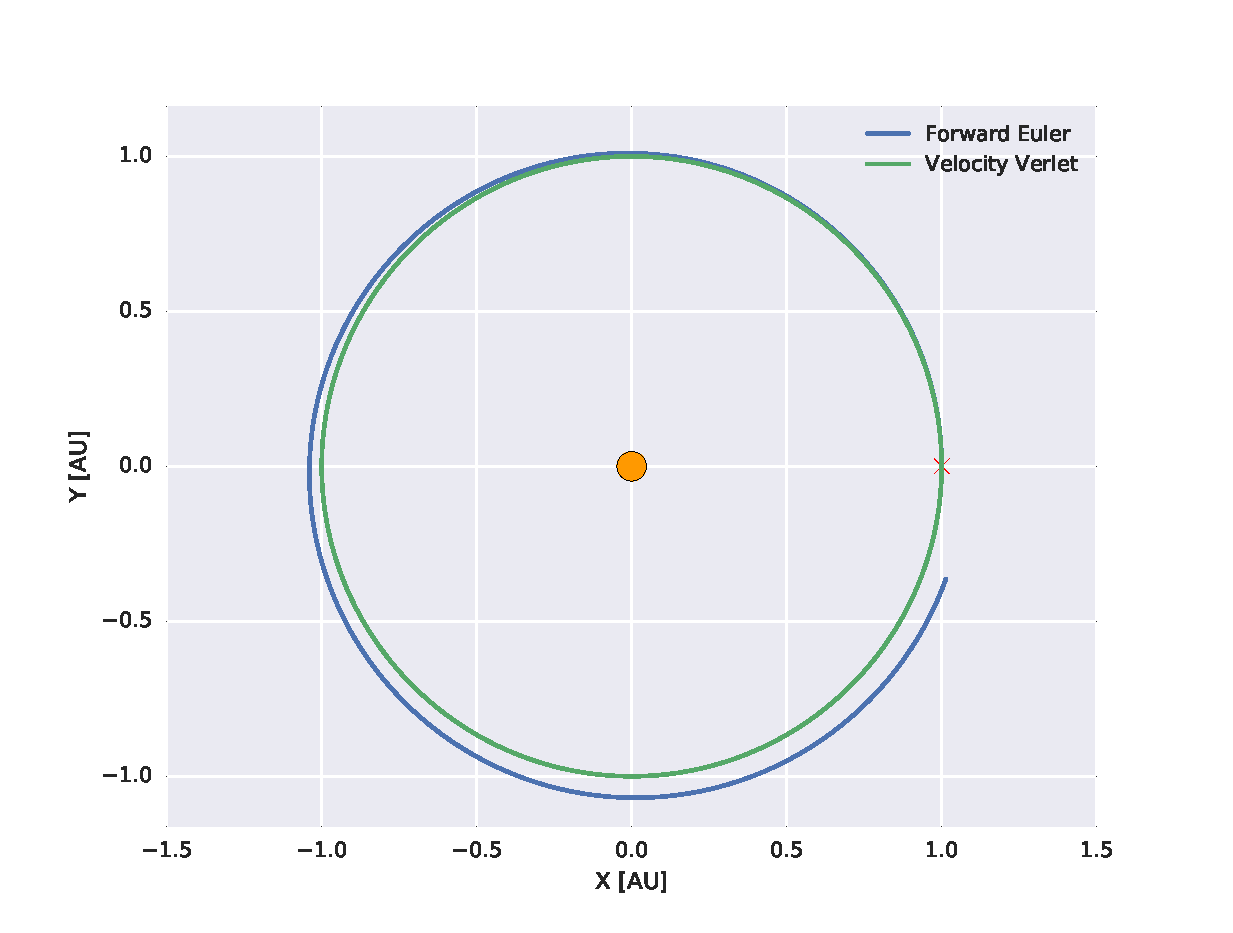
\includegraphics[width=\columnwidth]{figures/eulerverlet.eps}
  \caption{Position of the Earth forwarded for a year with the Euler and Verlet
  schemes. The initial position is marked with a red cross, and the initial
  velocity is in the positive y-direction.}
  \label{fig:earthsunorbits}
\end{figure}
The energies over time for both algorithms
are shown in figures~\ref{fig:eulerenergy} and~\ref{fig:verletenergy}.
\begin{figure}[H]
  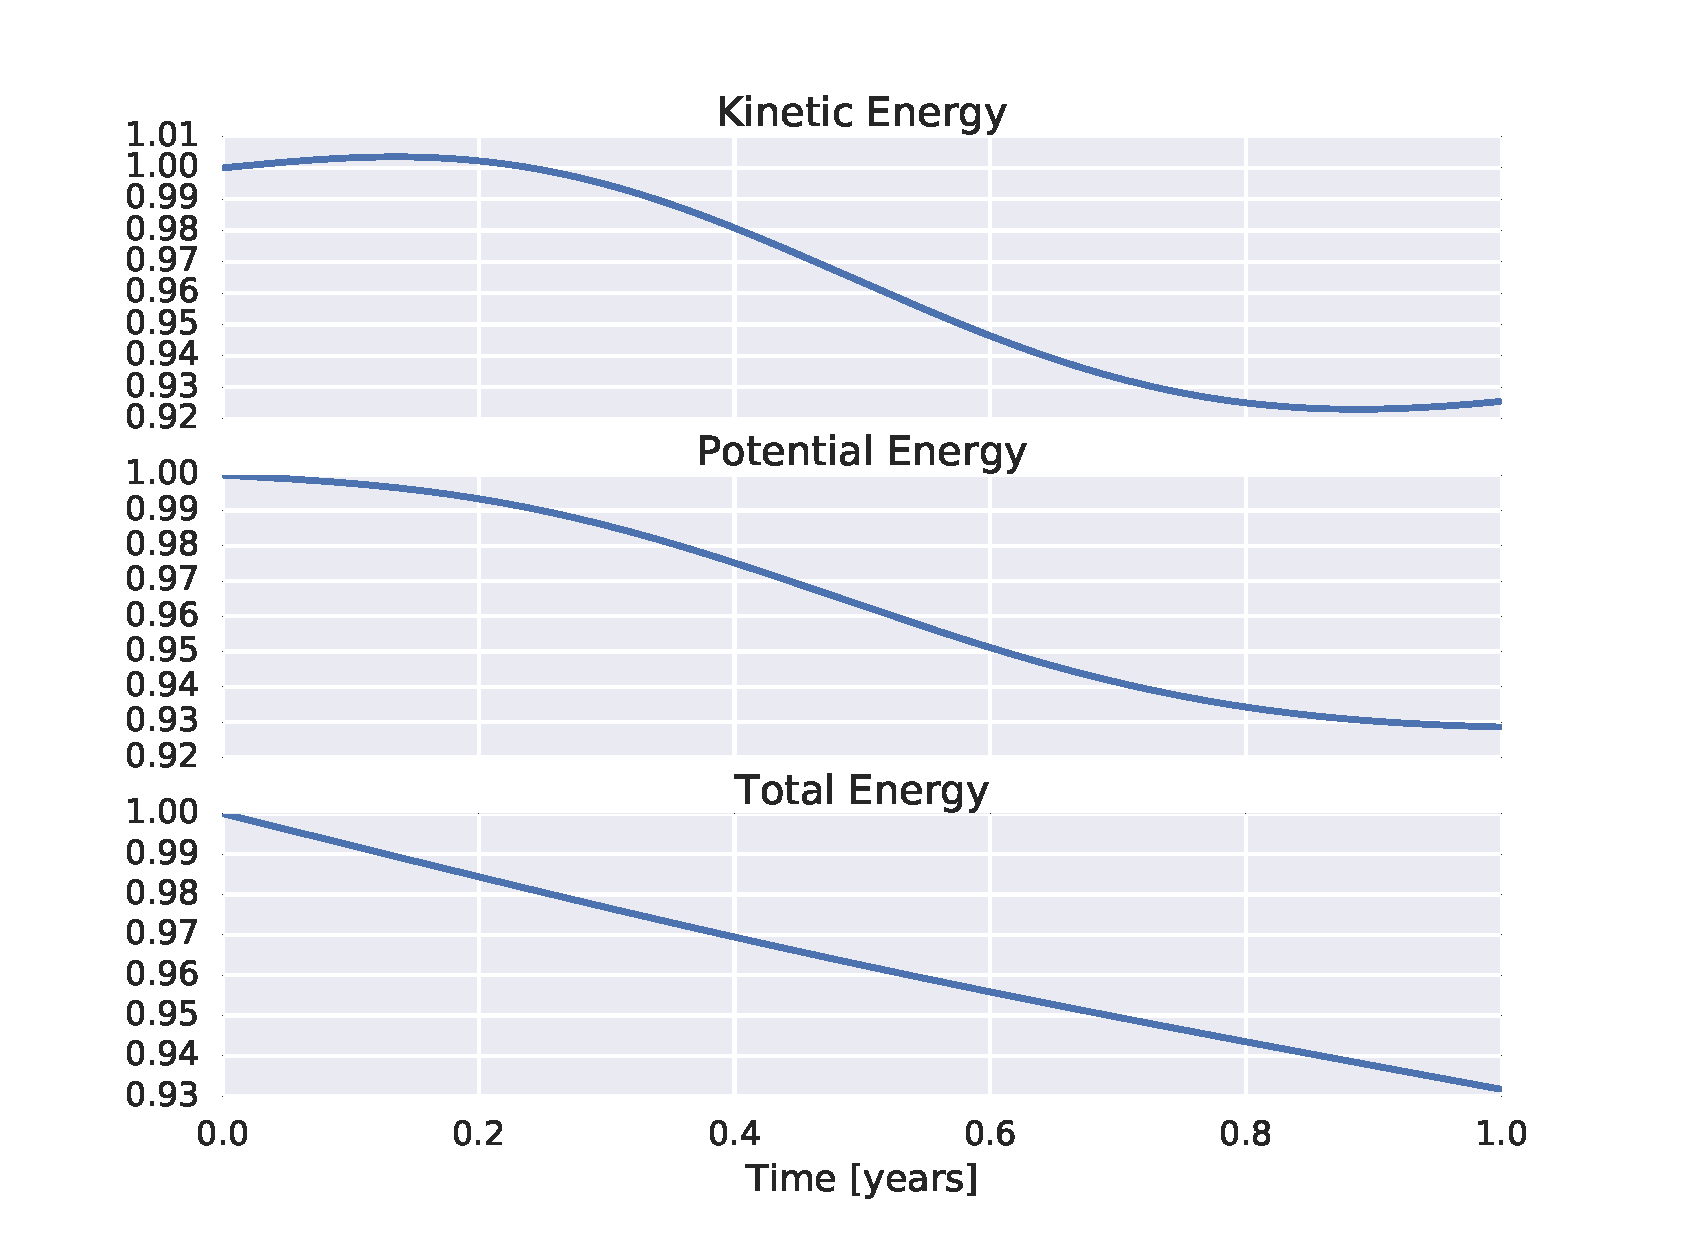
\includegraphics[width=\columnwidth]{figures/energy_euler.eps}
  \caption{Total energy over one year for the simple Earth-Sun system,
  forwarded with the Euler scheme. The distribution among kinetic and potential
  energy is also shown. The values are relative to the initial value.}
  \label{fig:eulerenergy}
\end{figure}

\begin{figure}[H]
  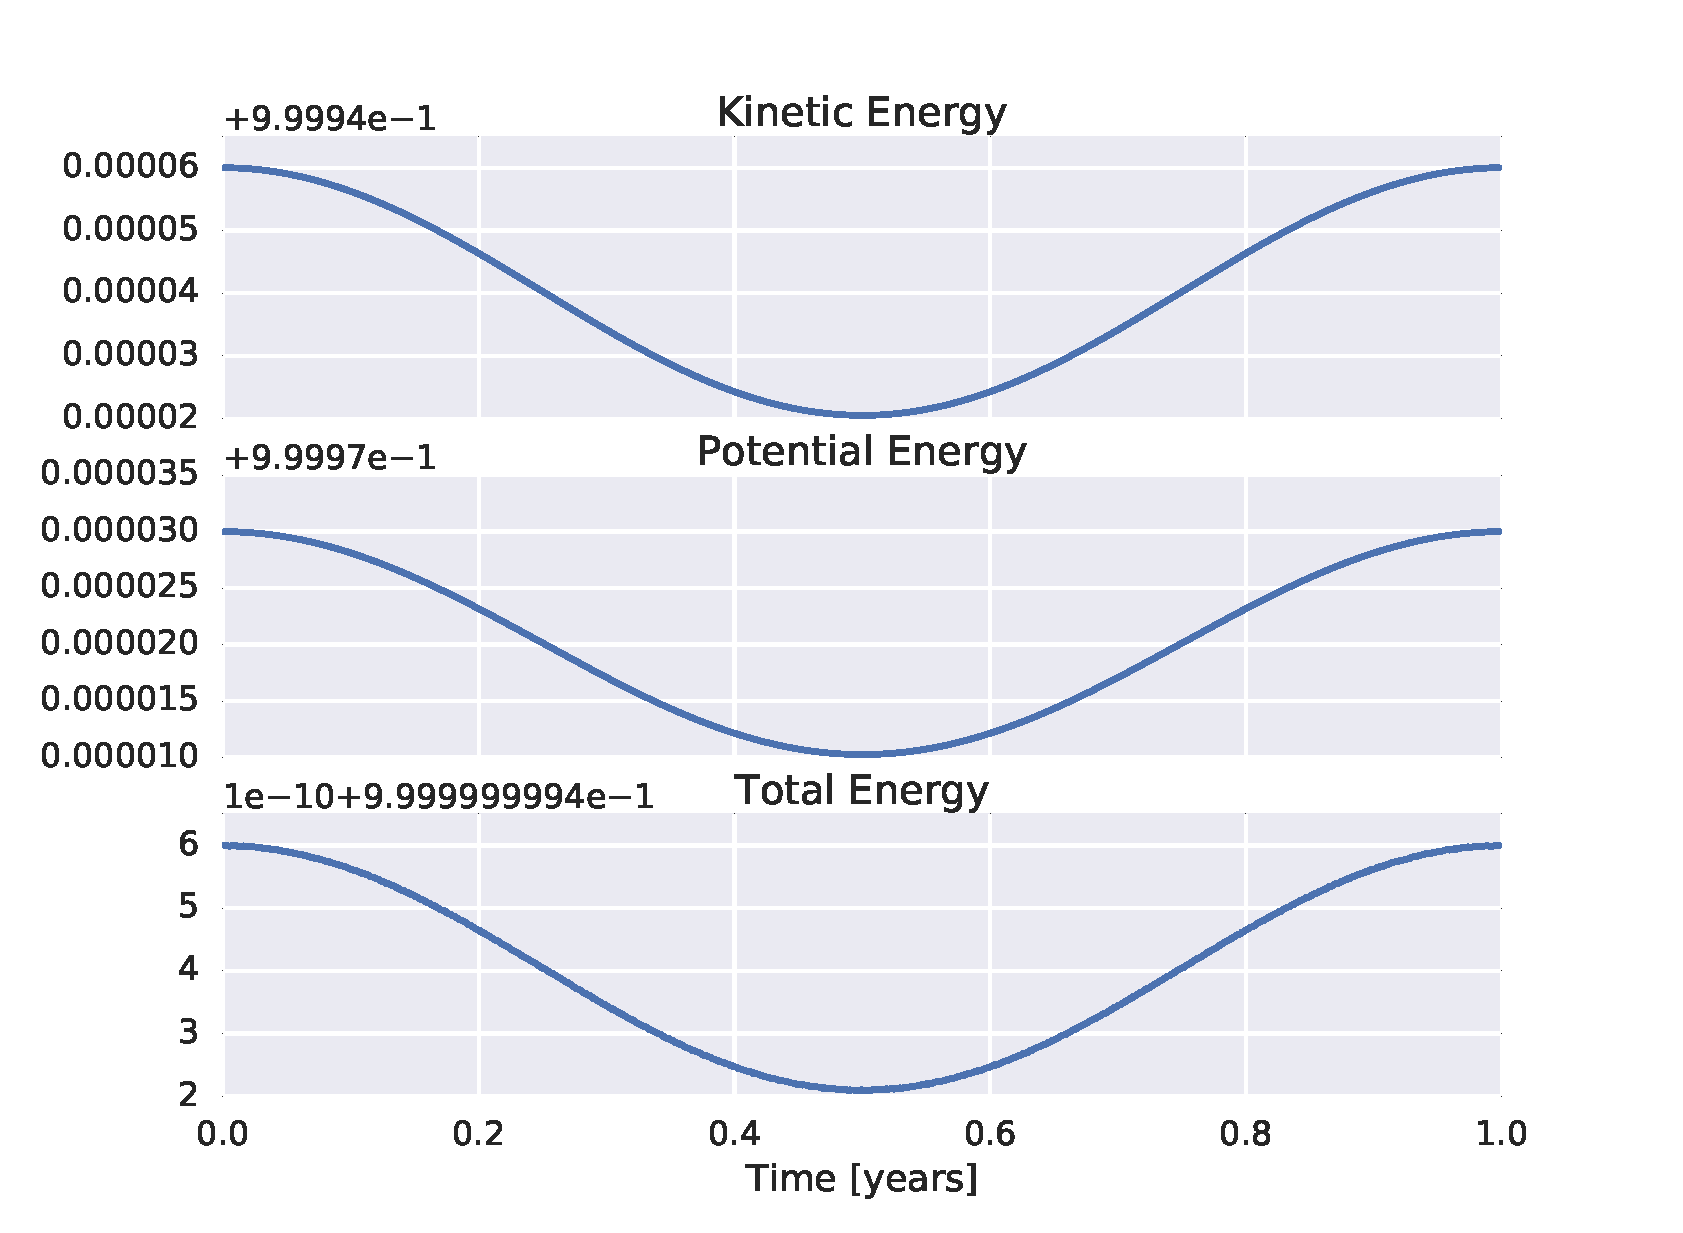
\includegraphics[width=\columnwidth]{figures/energy_verlet.eps}
  \caption{Total energy for one year for the Earth-Sun system, here forwarded
  with the Velocity Verlet solver.}
  \label{fig:verletenergy}
\end{figure}

For a comparison of the errors and computation timings for both algorithms, see
figure~\ref{fig:timing}.

\begin{figure}[H]
  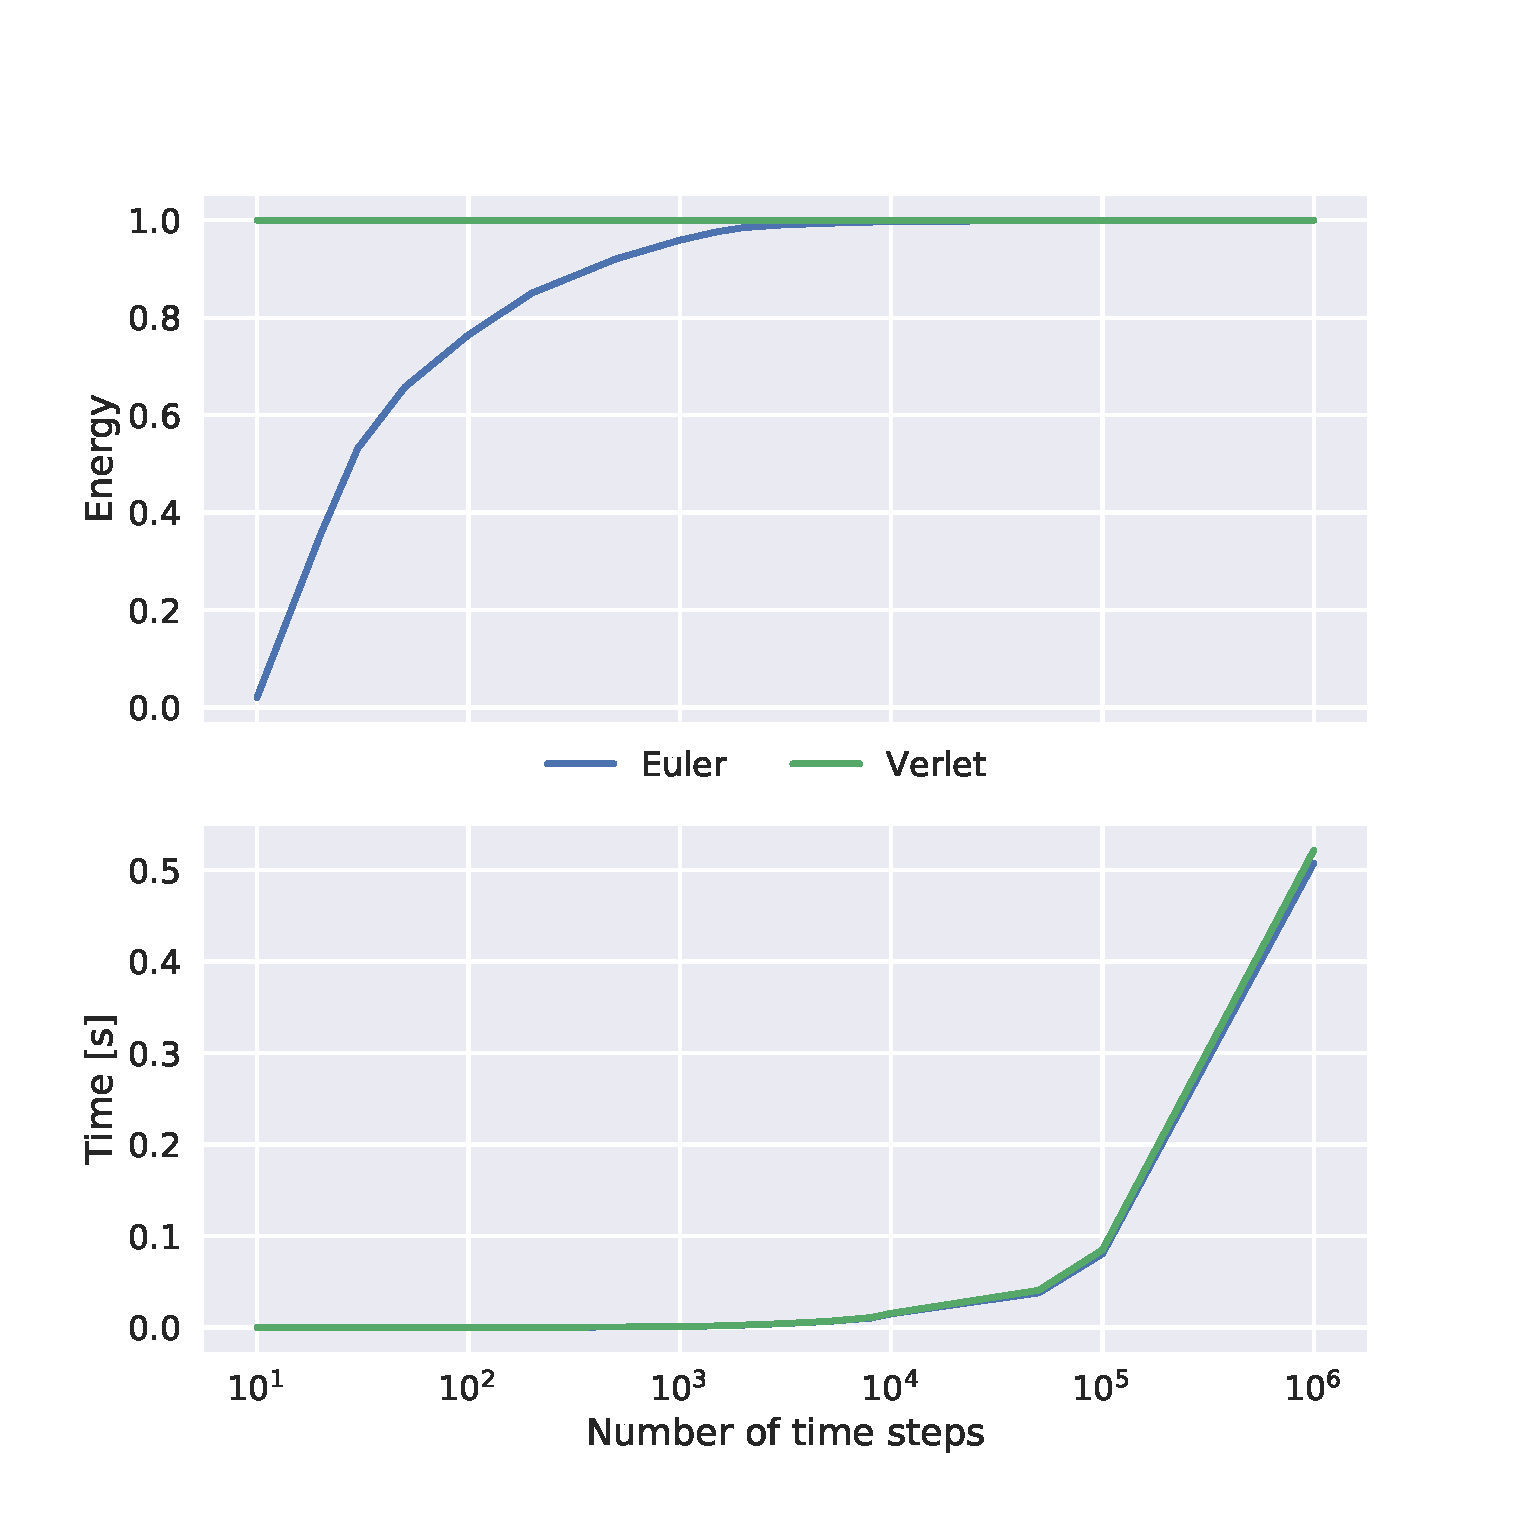
\includegraphics[width=\columnwidth]{figures/timing.eps}
  \caption{Comparison of the errors and timings for the co-planar one-year Earth-Sun
  simulation.}
  \label{fig:timing}
\end{figure}

\subsection{Escape velocity}

Figure~\ref{fig:escvel} shows the behavior of the convergence of the bisection
method for finding the escape velocity of the Earth-Sun system numerically. As
the number simulation period increases, the method converges to the analytical
expression.
\begin{figure}[H]
  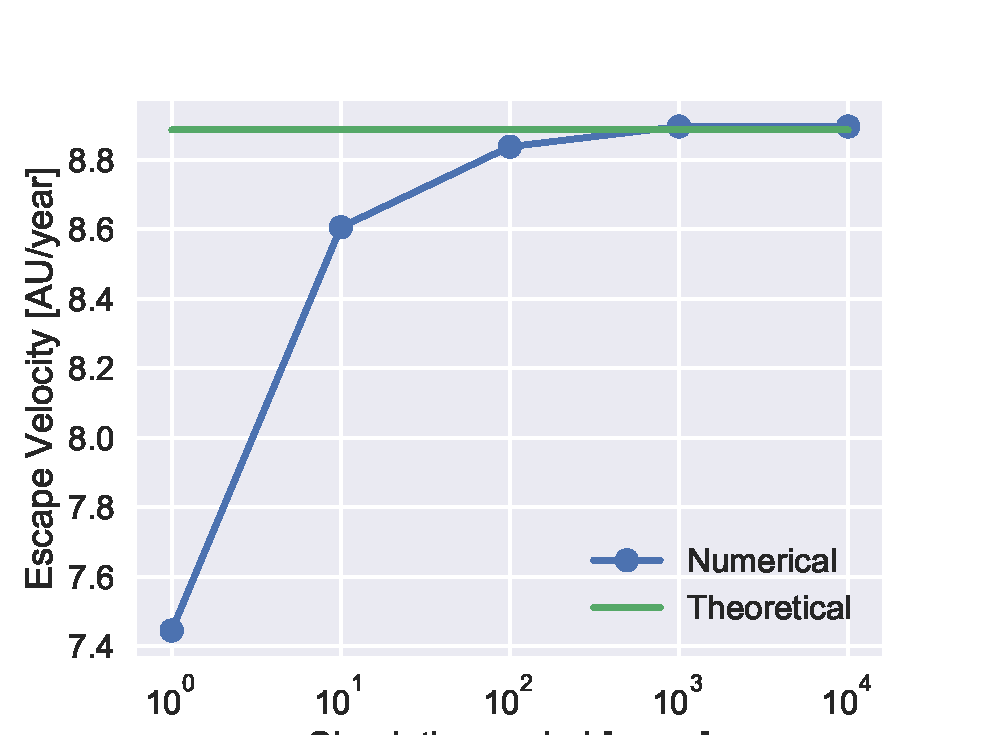
\includegraphics[width=\columnwidth]{figures/escapevelocity.eps}
  \caption{Numerically calculated escape velocities for different simulation
  periods. Notice the convergence to the analytical value.}
  \label{fig:escvel}
\end{figure}

As the exponent \(\beta\) in~\eqref{eq:duckling} was increased from \(2\) to
\(3\), the escape velocity decreased, as is visible from figure~\ref{fig:hei}.
\begin{figure}[H]
  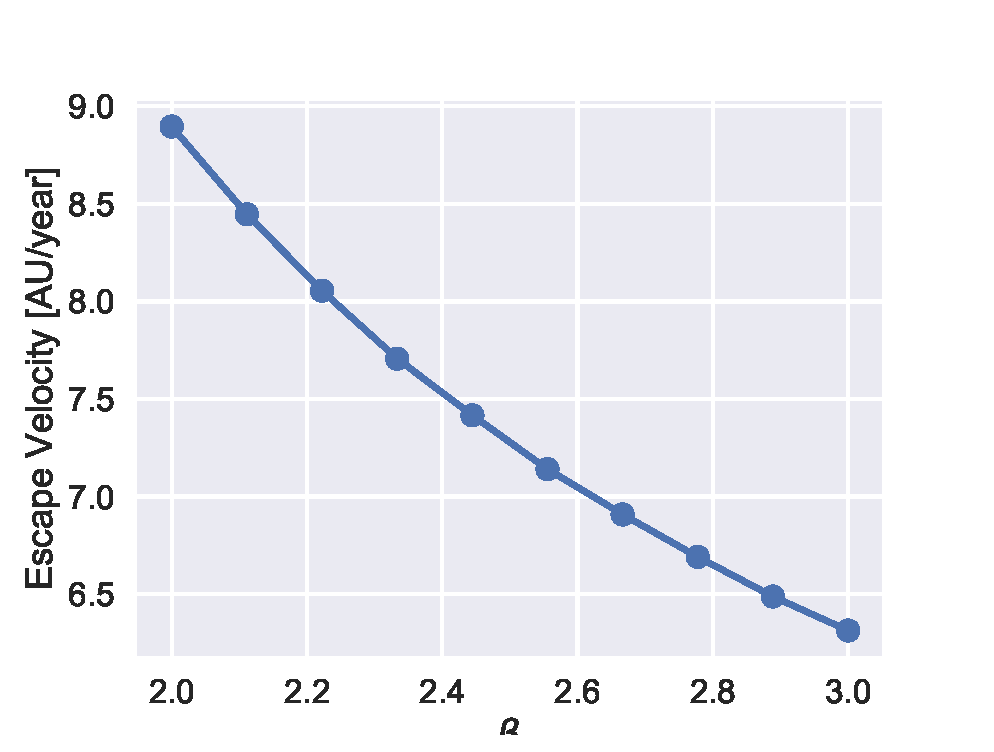
\includegraphics[width=\columnwidth]{figures/escapevelocitybeta.eps}
  \caption{Escape velocity calculated with the bisection method for different
  radius exponents $\beta$ in the Newtonian gravitational force expression.}
  \label{fig:hei}
\end{figure}

\subsection{Three-body problem}

The three-body problem was approximated with the Sun fixed or freely moving, and
where the mass of Jupiter was normal, ten times as large or a hundred times as
large. Figure~\ref{fig:animals} shows the results.
\begin{figure}
  \begin{tabular}{cc}
    \centering
    \begin{subfigure}[b]{0.5\columnwidth}
        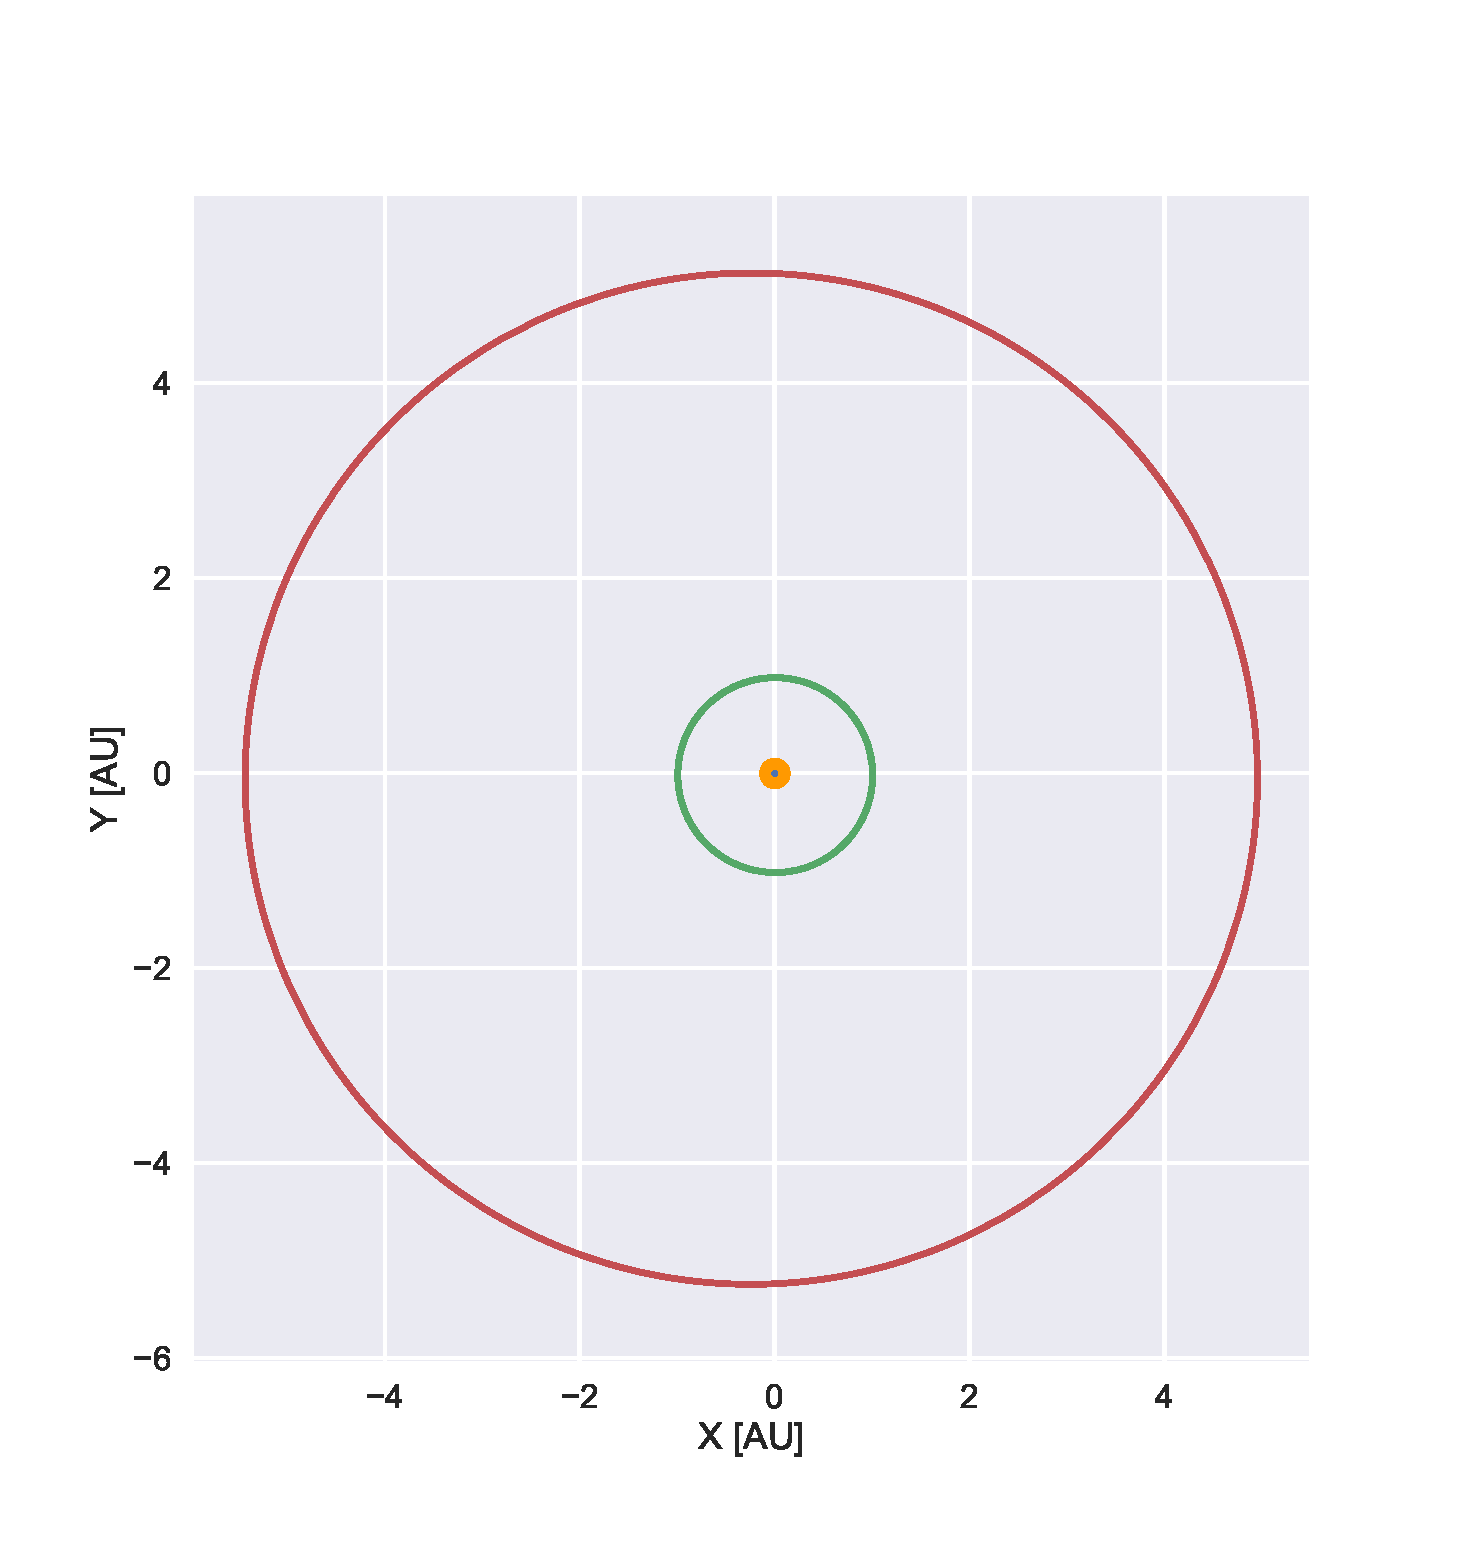
\includegraphics[width=\columnwidth]{figures/jupiter_1.eps}
        \caption{Fixed sun with a normal Jupiter mass}
        \label{fix1}
    \end{subfigure}&
    \begin{subfigure}[b]{0.5\columnwidth}
        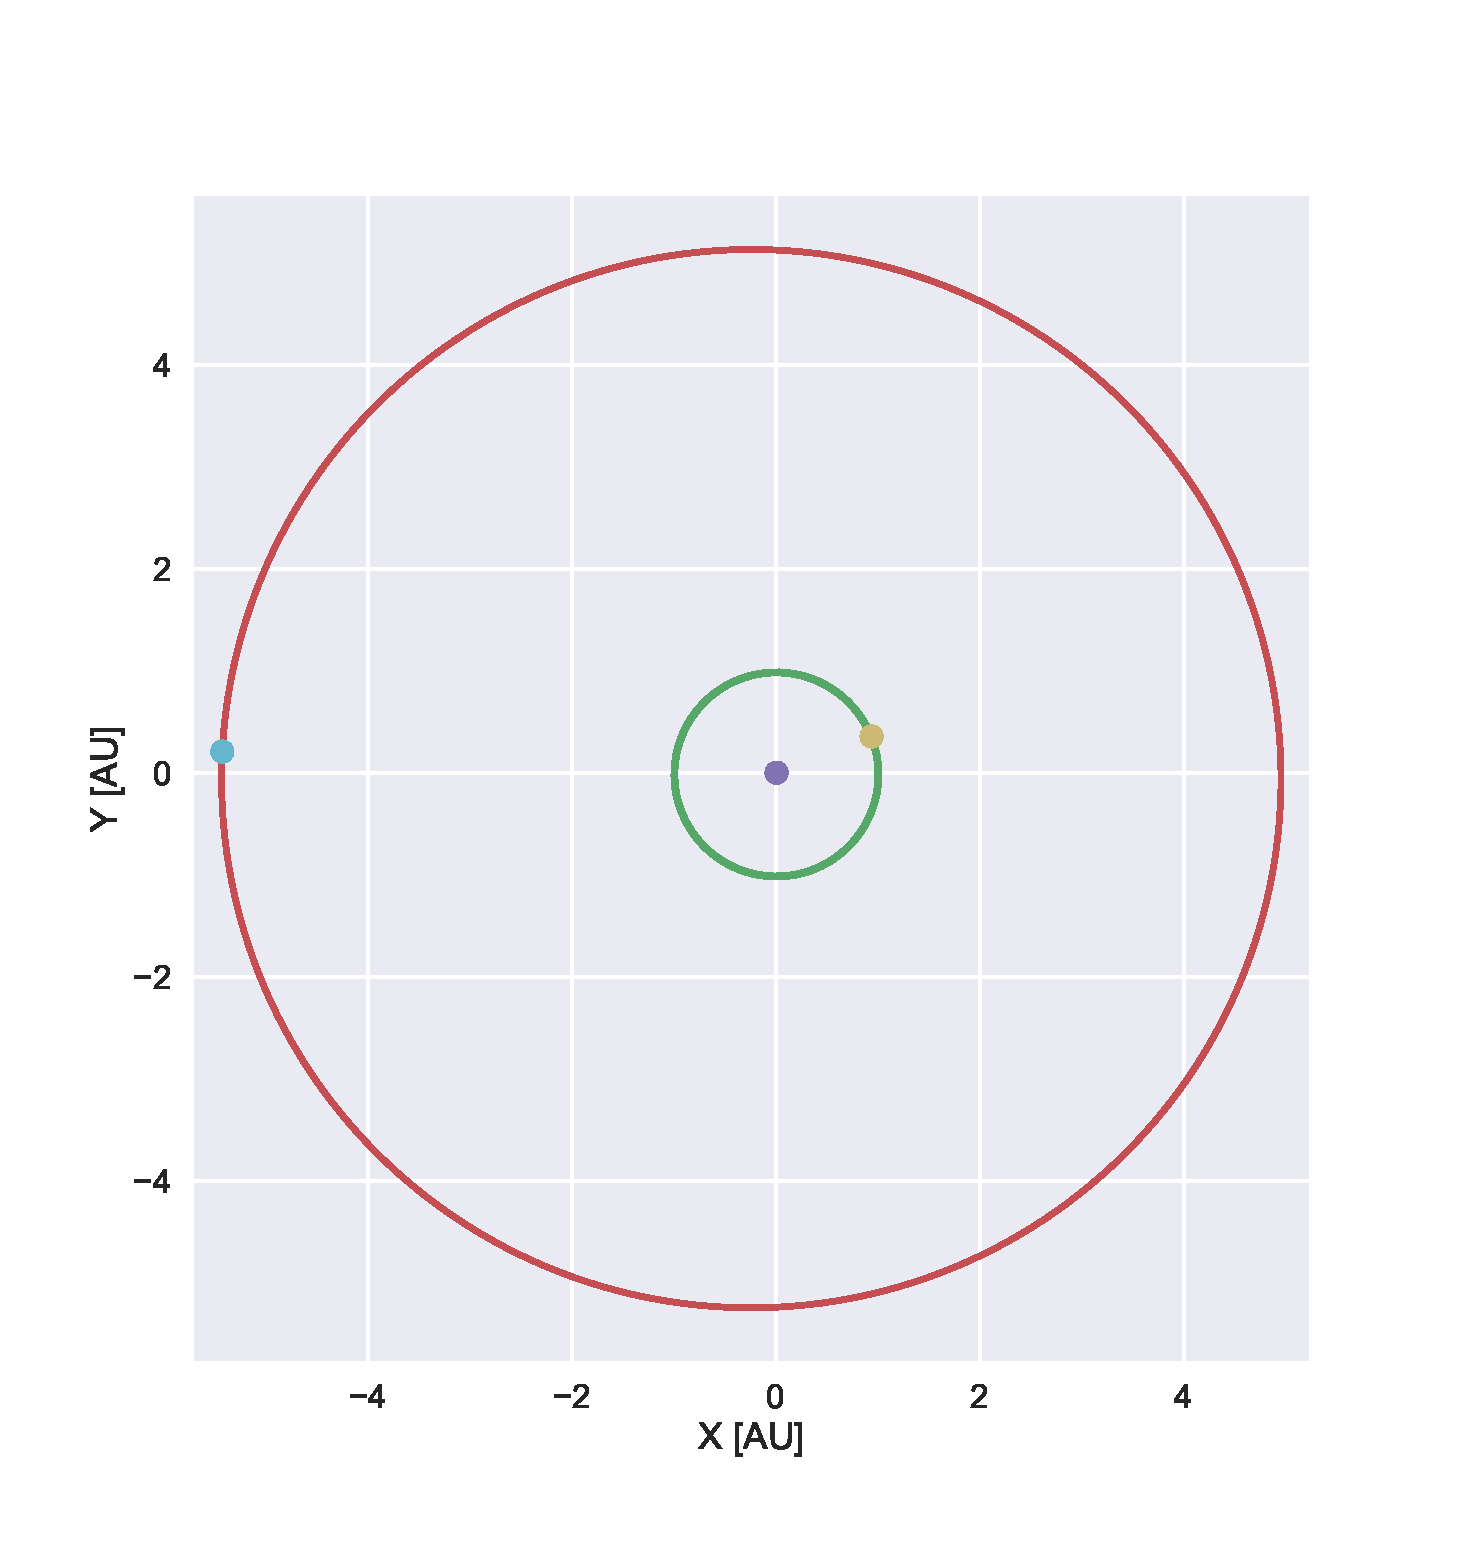
\includegraphics[width=\columnwidth]{figures/jupiter2_1.eps}
        \caption{Free sun with a normal Jupiter mass}
        \label{free1}
    \end{subfigure}\\
    \begin{subfigure}[b]{0.5\columnwidth}
      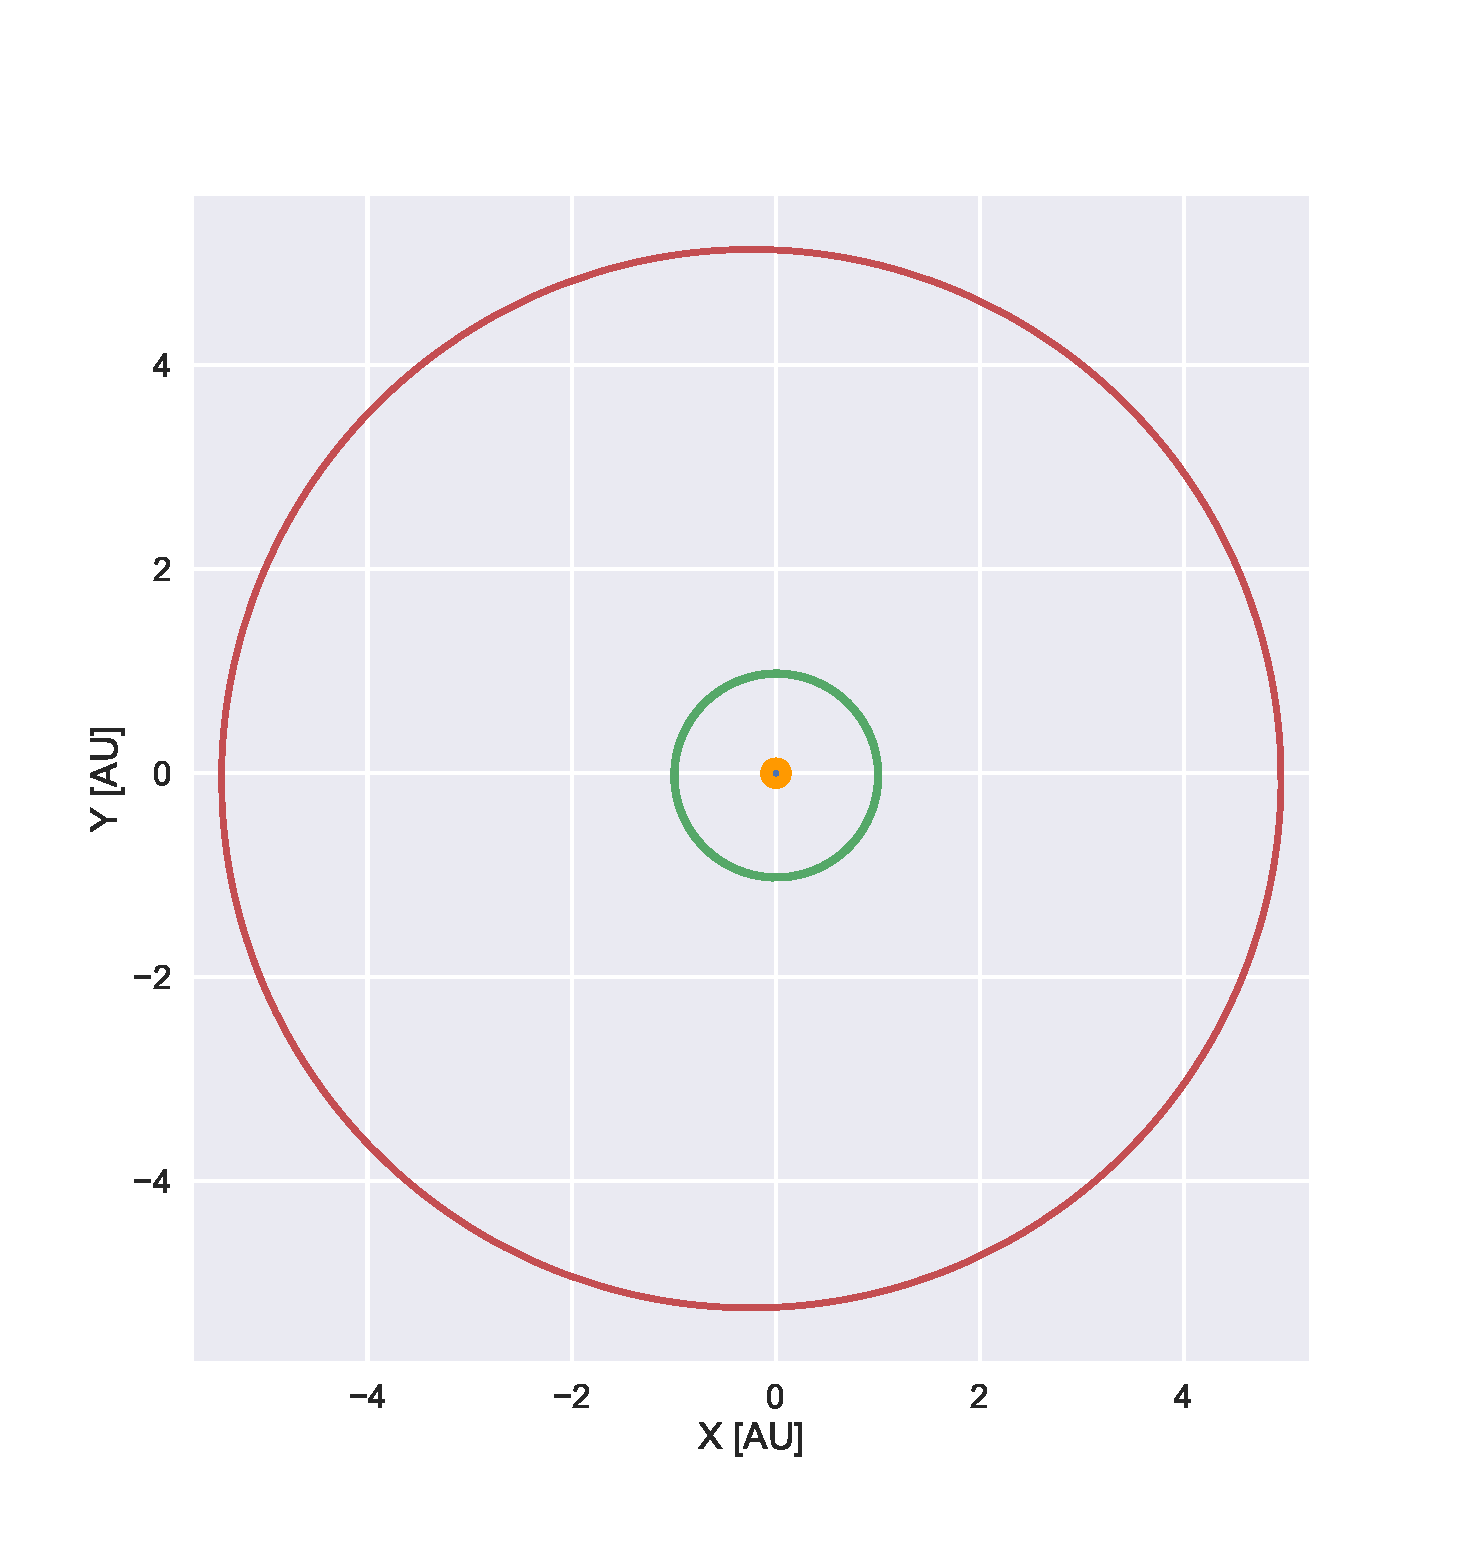
\includegraphics[width=\columnwidth]{figures/jupiter_10.eps}
        \caption{Fixed sun with a \(10x\) Jupiter mass}
        \label{fix10}
    \end{subfigure}&
    \begin{subfigure}[b]{0.5\columnwidth}
        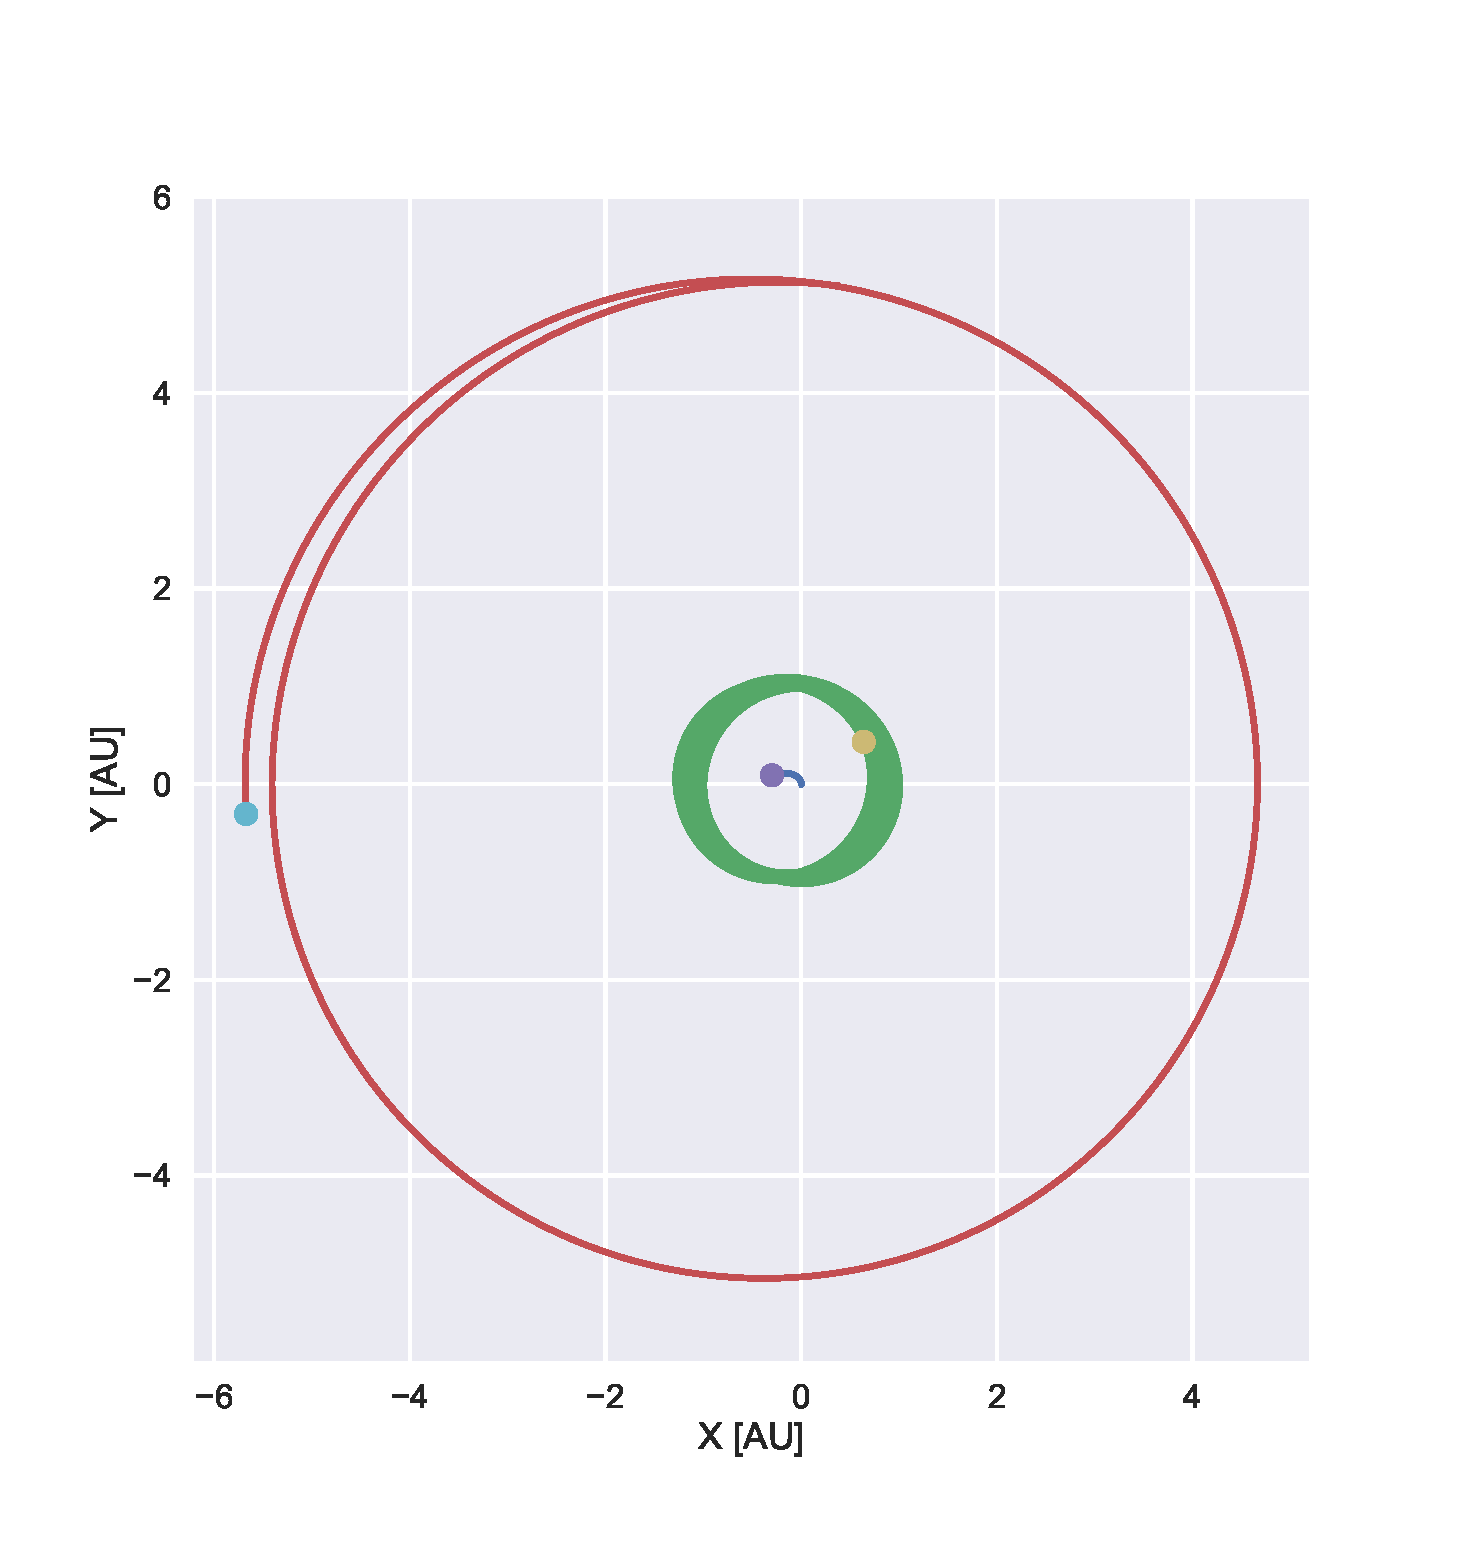
\includegraphics[width=\columnwidth]{figures/jupiter2_10.eps}
        \caption{Free sun with a \(10x\) Jupiter mass}
        \label{free10}
    \end{subfigure}\\
    \begin{subfigure}[b]{0.5\columnwidth}
        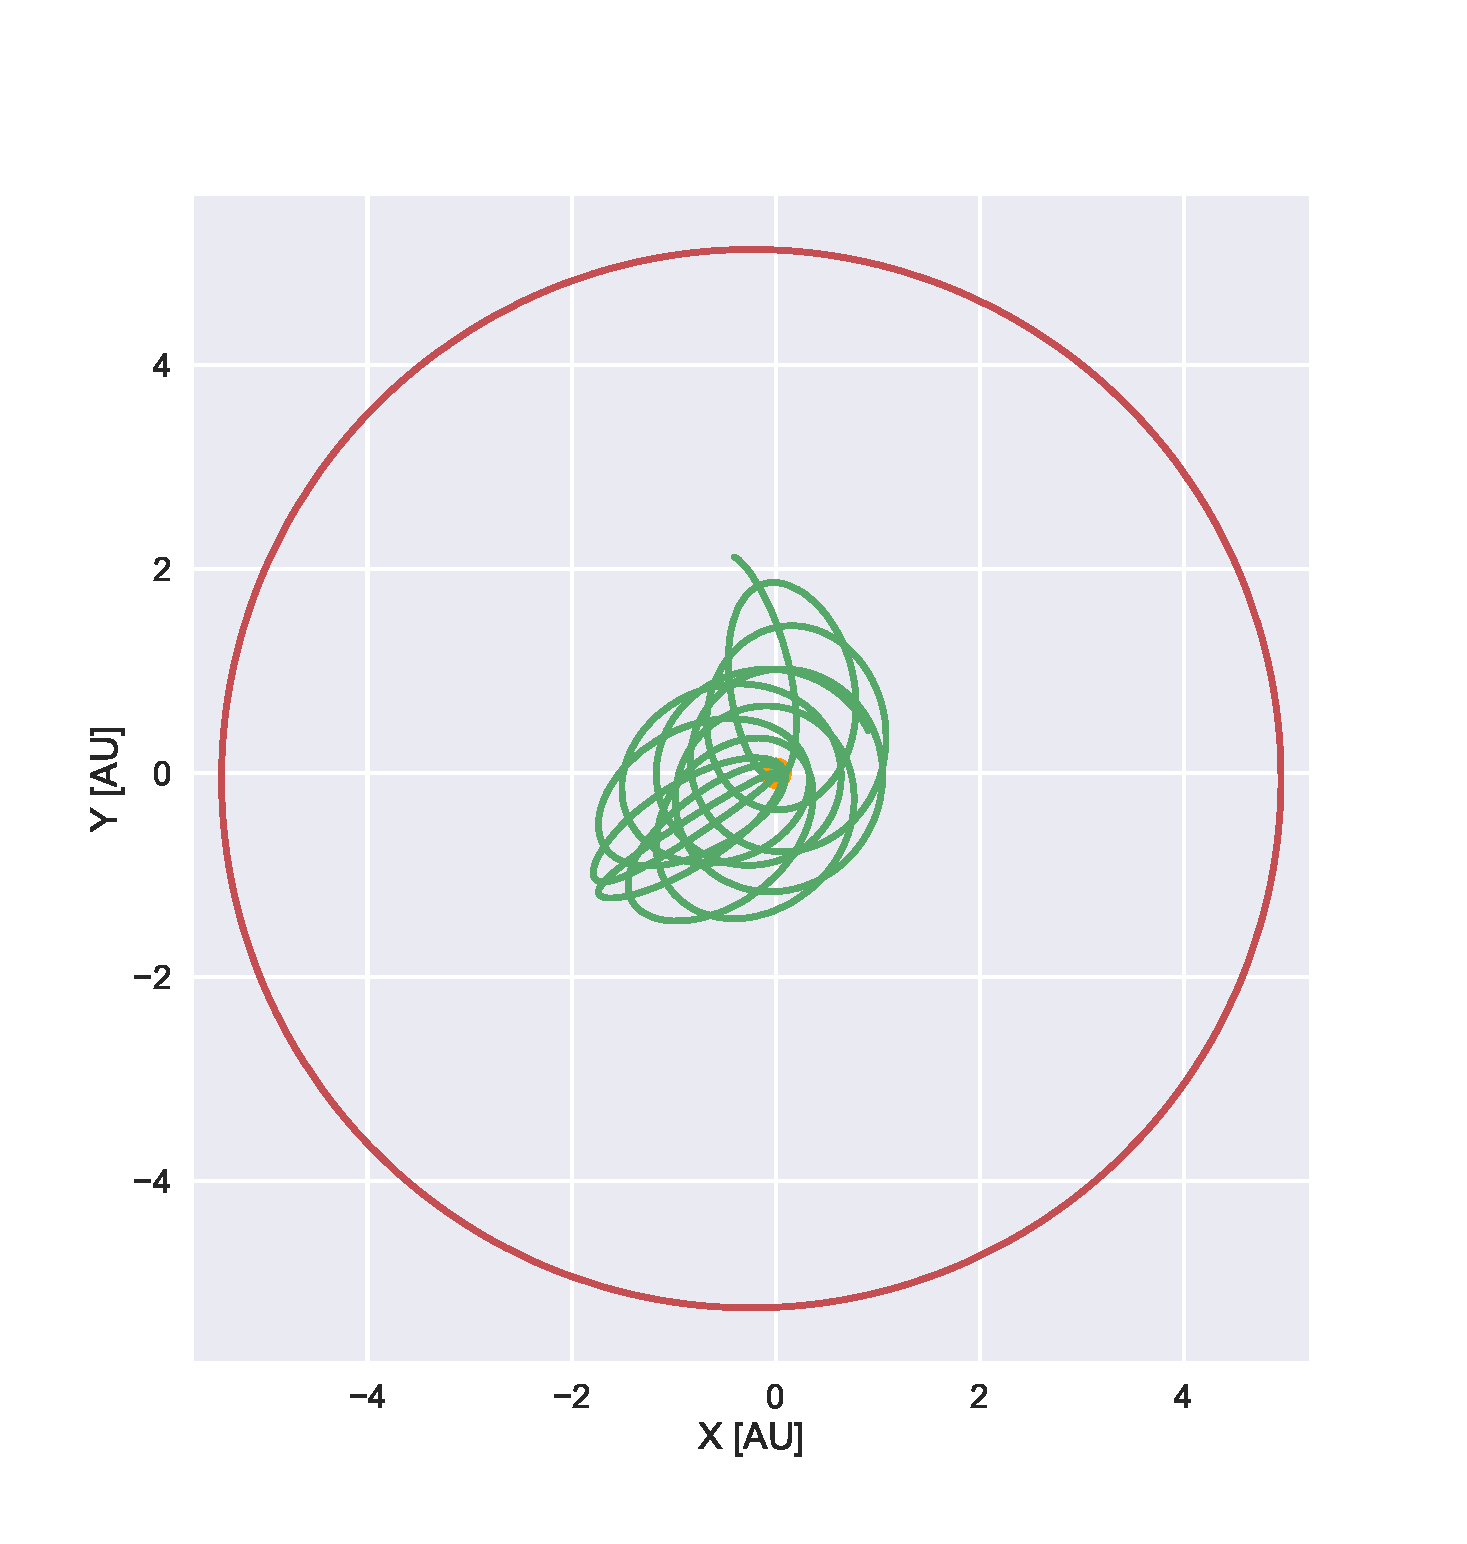
\includegraphics[width=\columnwidth]{figures/jupiter_100.eps}
        \caption{Fixed sun with a \(1000x\) Jupiter mass}
        \label{fix1000}
    \end{subfigure}&
    \begin{subfigure}[b]{0.5\columnwidth}
      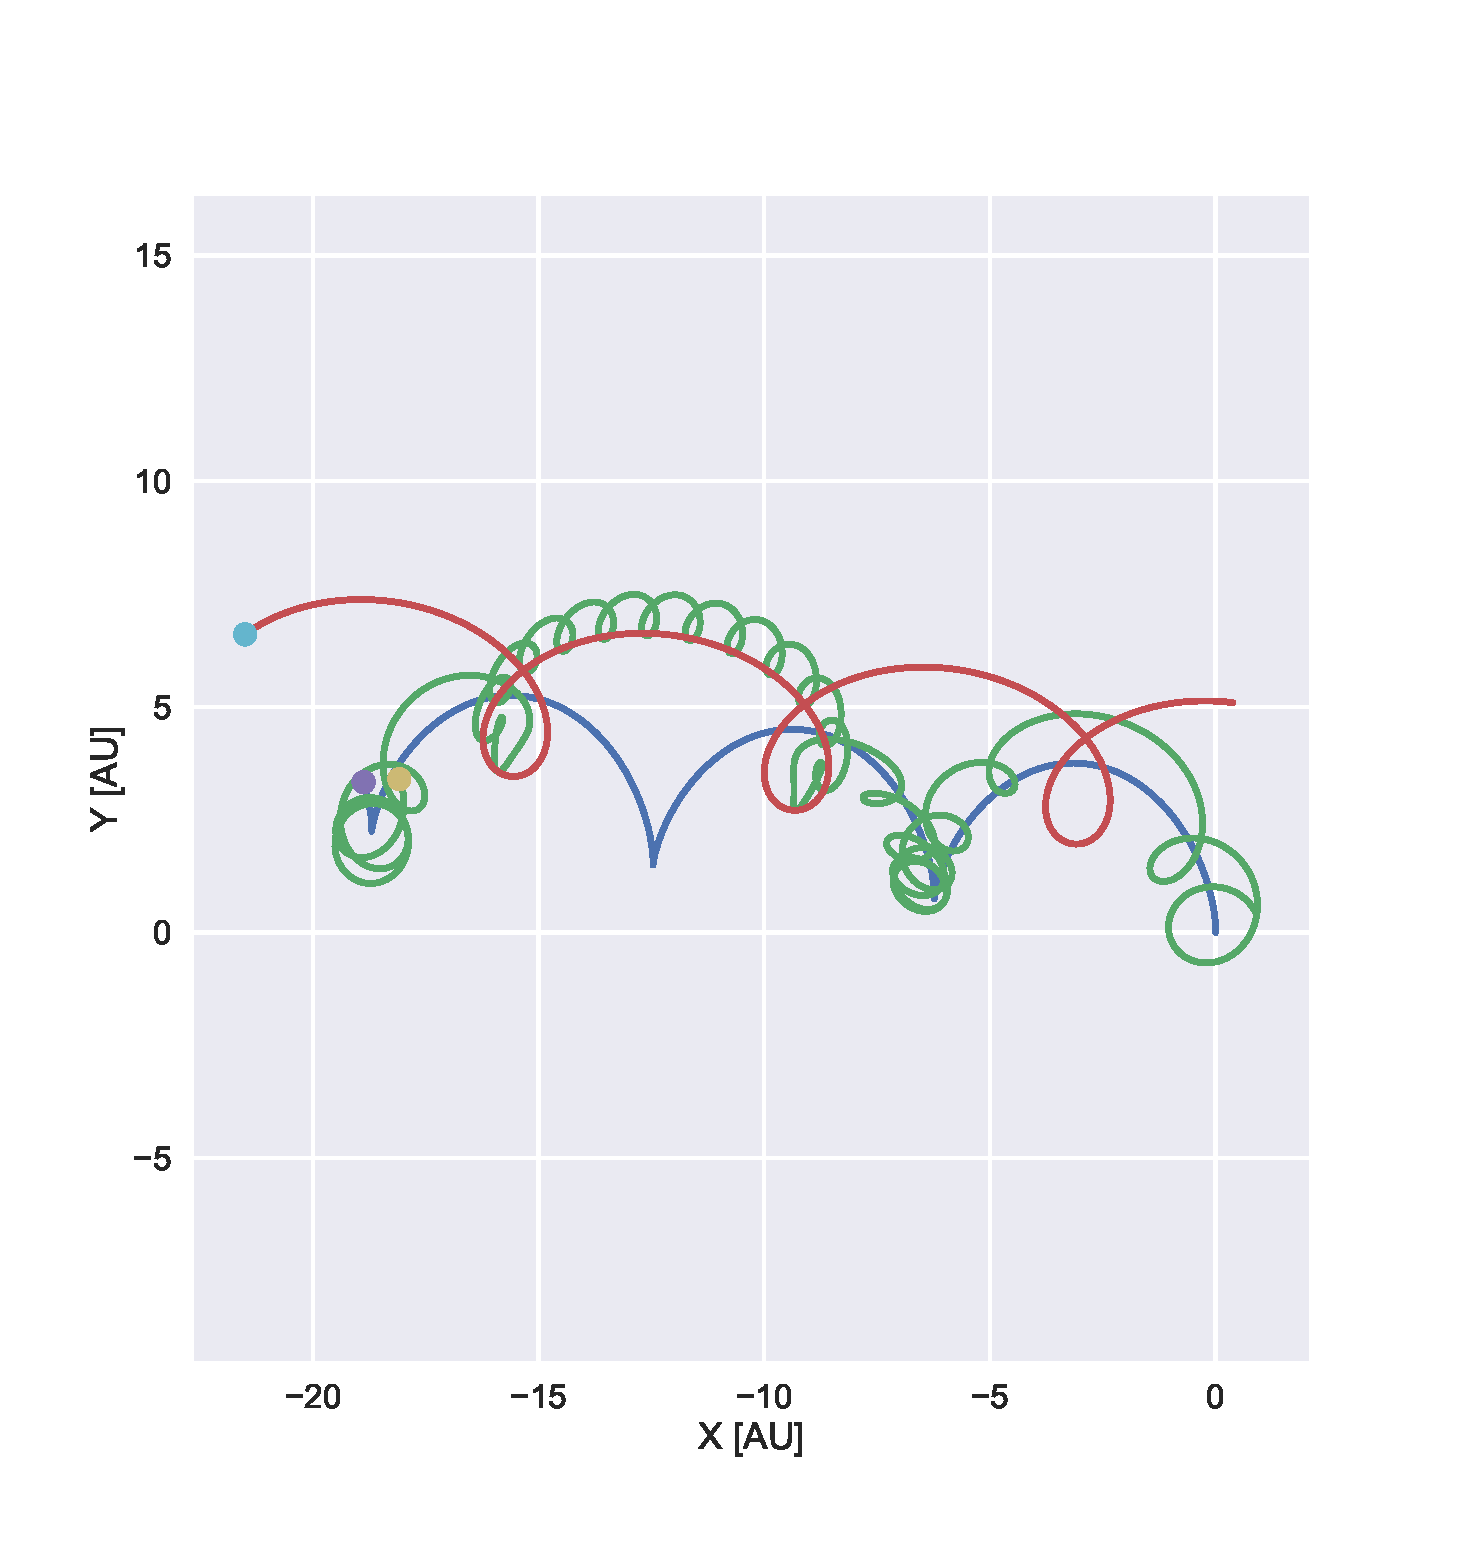
\includegraphics[width=\columnwidth]{figures/jupiter2_100.eps}
        \caption{Free sun with a \(1000x\) Jupiter mass}
        \label{free1000}
    \end{subfigure}\\
    \end{tabular}
    \caption{The numerical solutions for the three body problem under different parameters.}\label{fig:animals}
\end{figure}

\subsection{Full solar system simulation}

A system of the full solar system was performed for a period of \(12\) years in
three dimensions. The resulting plot is shown is figure~\ref{fig:fullsystem}.
Figures~\ref{fig:fullsystemenergy} and~\ref{fig:fullsystemang} shows the
relative energy and angular momentum of the system.

\begin{figure}[H]
  \centering
  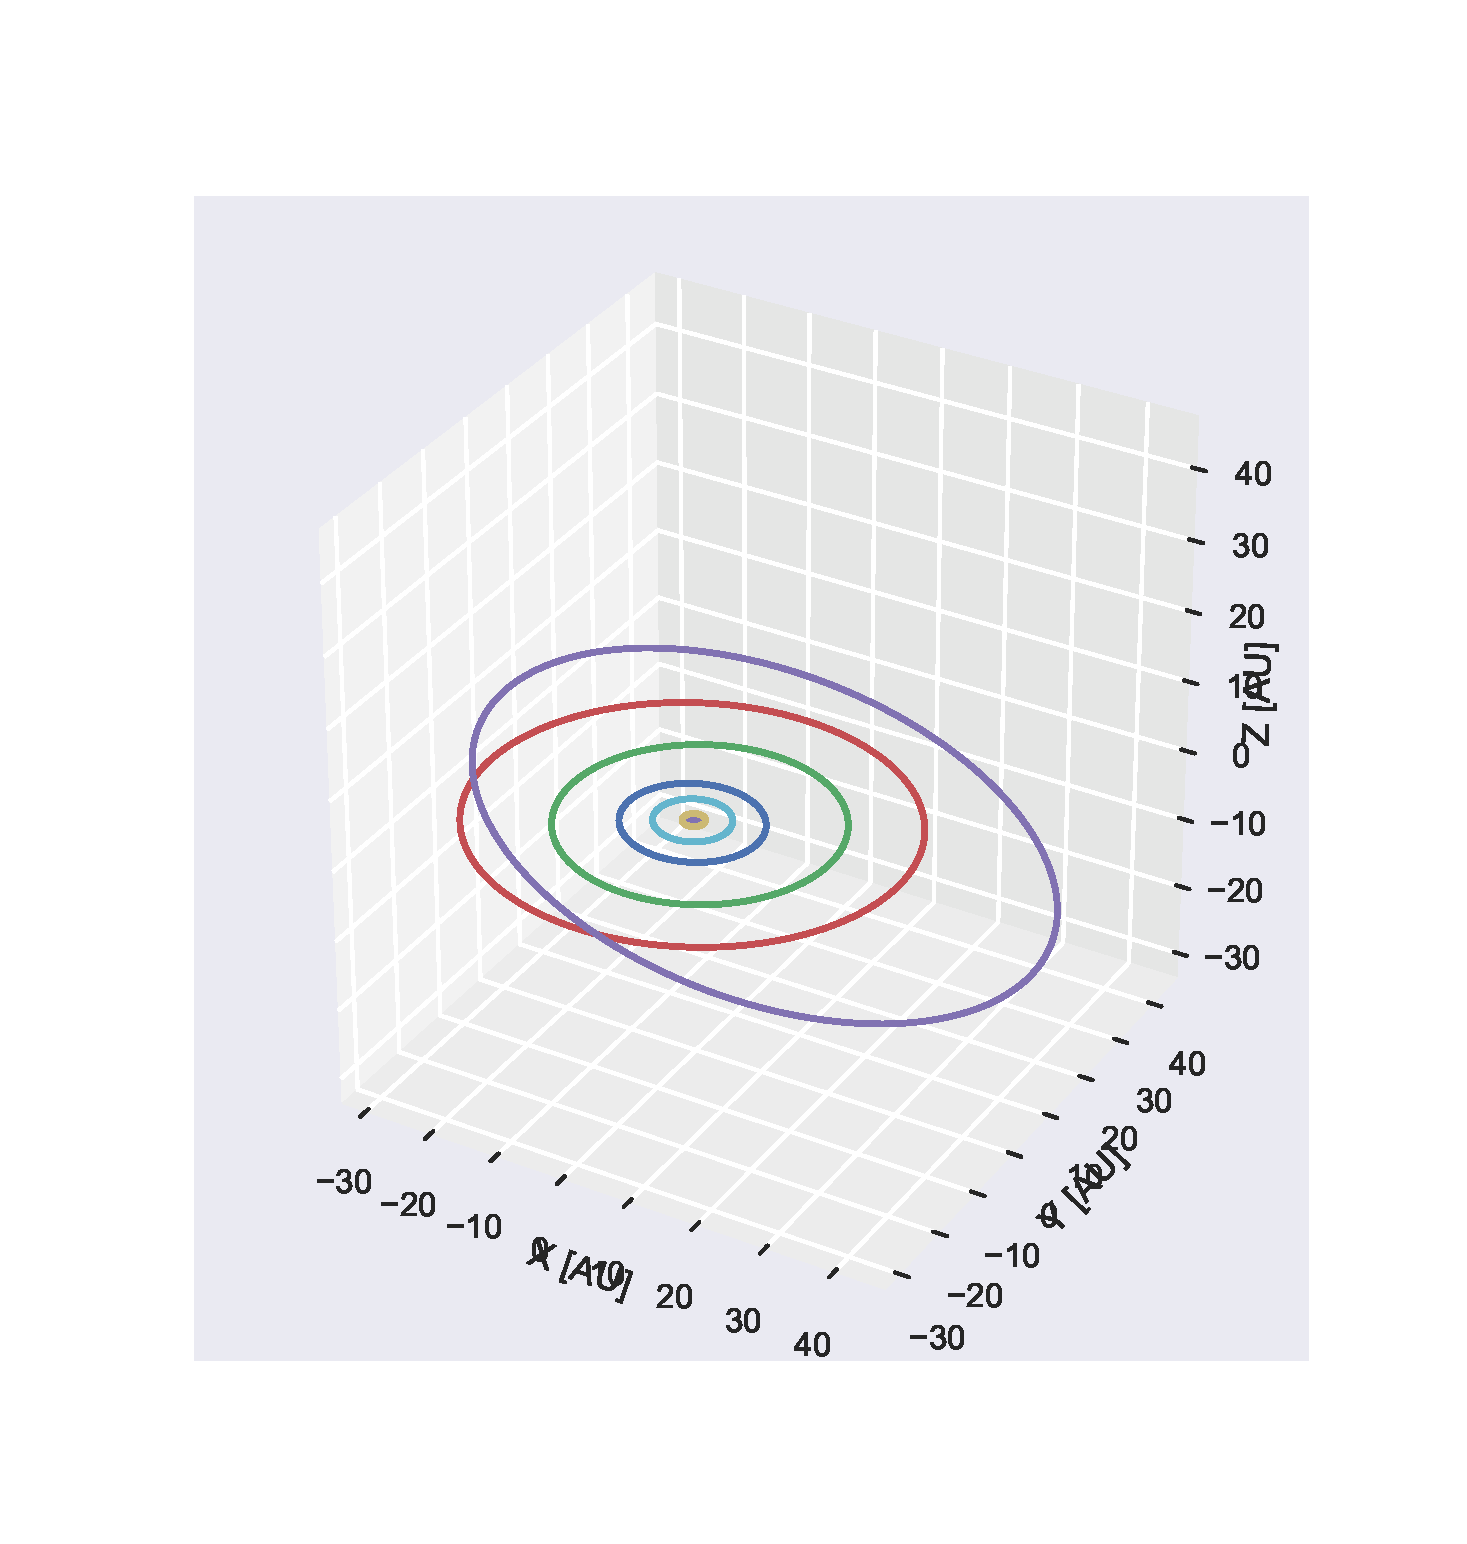
\includegraphics[width=\columnwidth]{figures/fullsystem.eps}
  \caption{\label{fig:fullsystem} The evolution of the solar system as time
    progresses over a period of \(300\) years.}
\end{figure}

\begin{figure}[H]
  \centering
  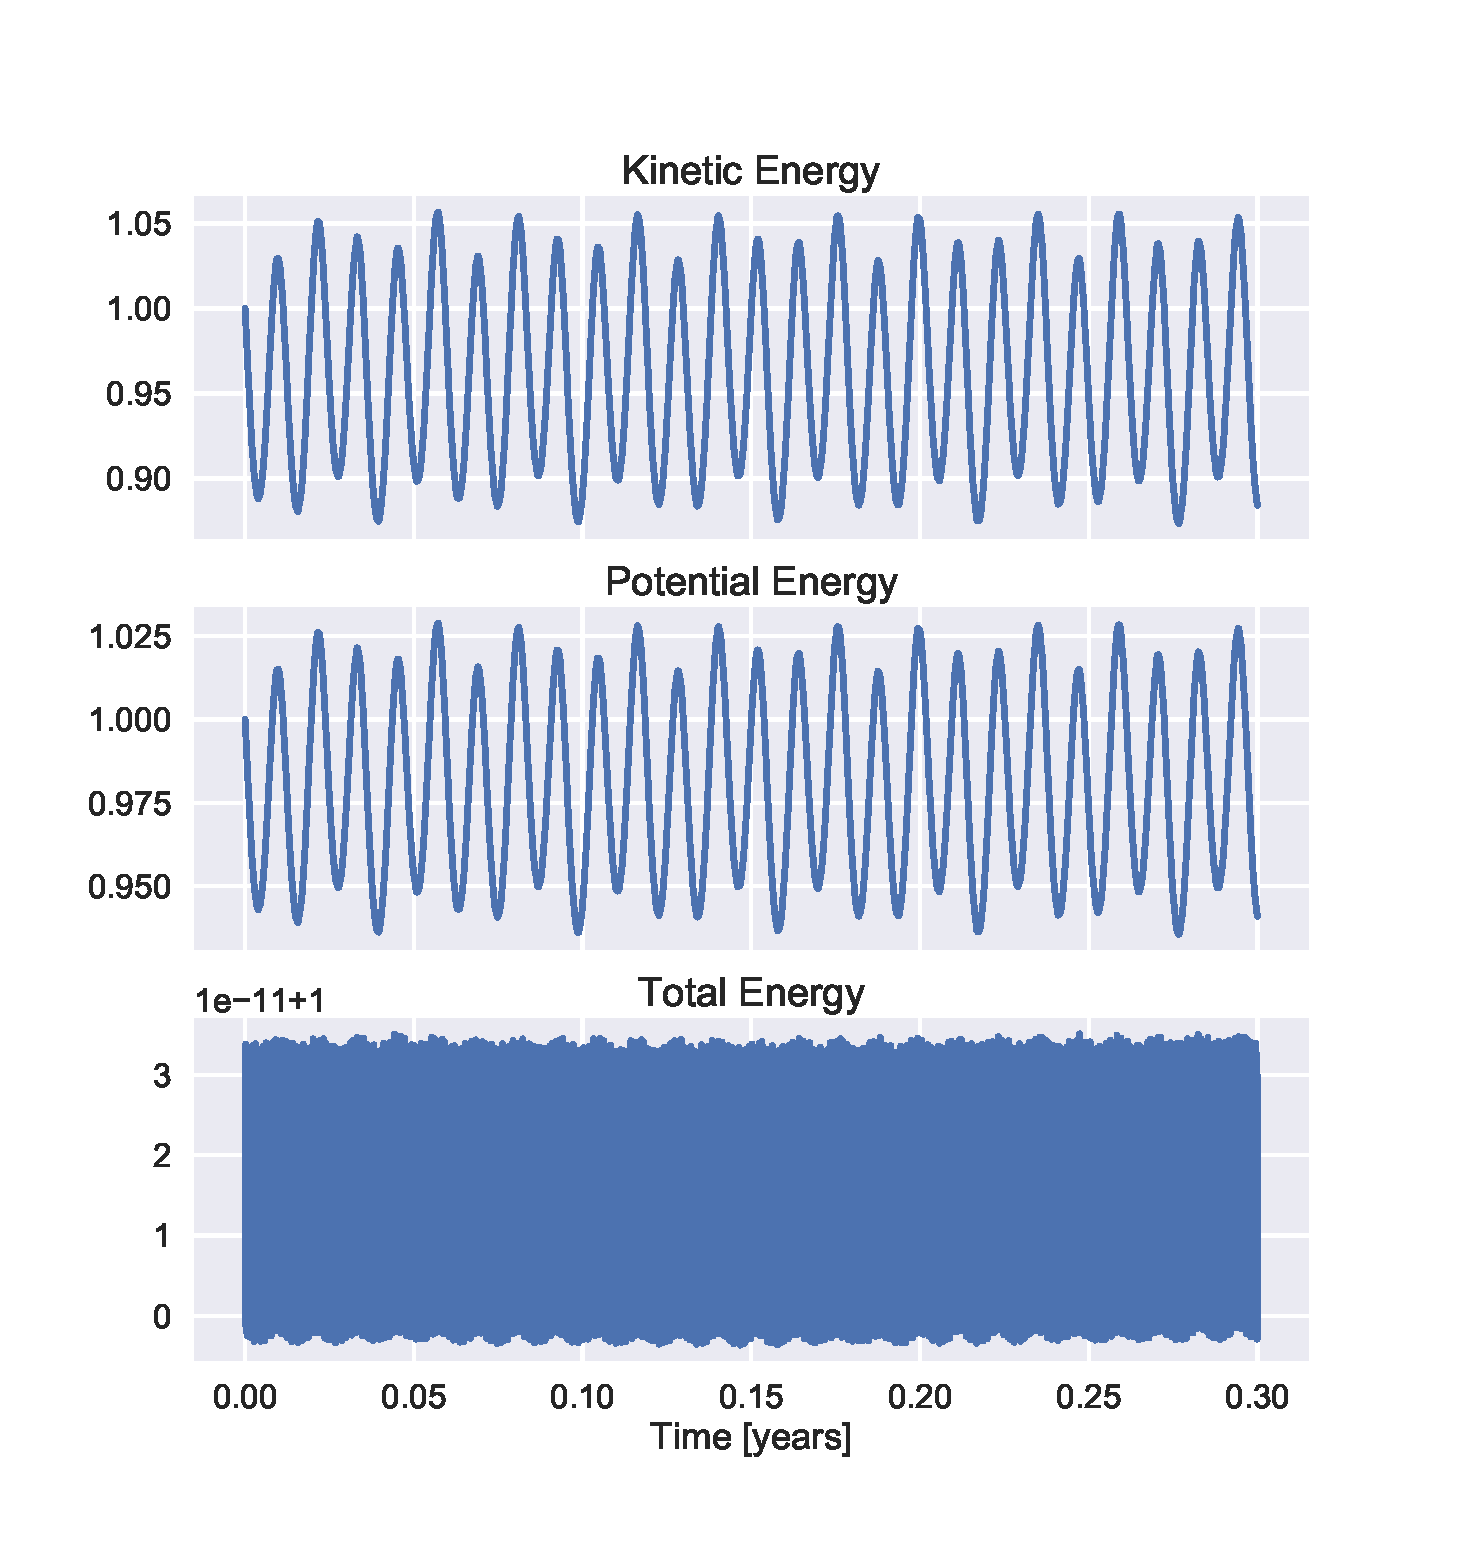
\includegraphics[width=\columnwidth]{figures/fullsystem_energy.eps}
  \caption{\label{fig:fullsystemenergy} The change in relative energy
    of the solar system.}
\end{figure}

\begin{figure}[H]
  \centering
  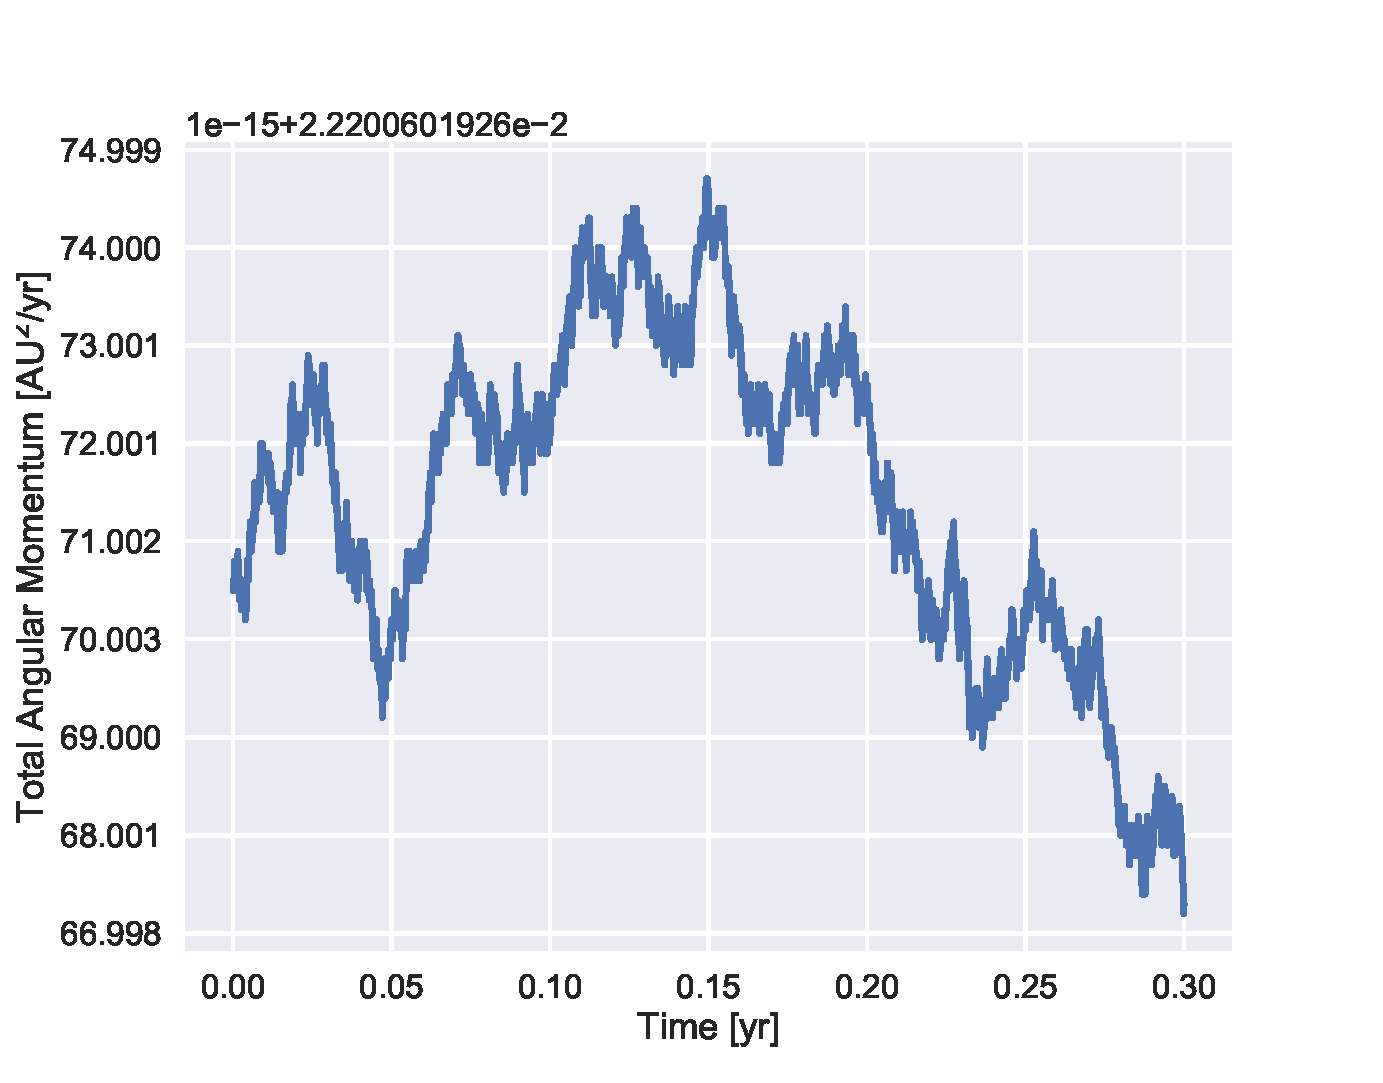
\includegraphics[width=\columnwidth]{figures/fullsystem_ang.eps}
  \caption{\label{fig:fullsystemang} The change in angular momentum of the solar
  system.}
\end{figure}


\subsection{The perihelion precession of Mercury}

The perihelion precession of Mercury is shown in figures~\ref{fig:newtonper}
and~\ref{fig:relatper} for pure Newtonian Mechanics and with relativistic
correction, respectively. These were produced by using \(10^{7}\) steps per year.

\begin{figure}[H]
  \centering
  \includegraphics[width=\columnwidth]{figures/newtonprecession.eps}
  \caption{\label{fig:newtonper} The precession of Mercury over a century with
    pure Newtonian mechanics.}
\end{figure}

\begin{figure}[H]
  \centering
  \includegraphics[width=\columnwidth]{figures/precession.eps}
  \caption{\label{fig:relatper} The precession of Mercury over a century using
    the relativistic correction.}
\end{figure}


\section{Discussion}
\label{sec:discussion}
The results from the previous section are discussed systimatically in the order
presented.
\subsection{Earth-Sun system}
Because of the simplicity of the Earth-Sun system, a detailed comparison of the
algorithms is possible. The expected analytical behaviour is also trivial to
find, which makes proper error analysis possible. By inspection of the figure with the
planet positions, it is evident that the Velocity Verlet method outperforms
the Euler method in terms of accuracy. Notice that the Verlet method computes what
appears a complete orbit, as expected for the Earth with the given initial conditions.
With the Euler method, the Earth visibly spirals outwards with time.

The difference is also very clear from the energy figures. With the Verlet
implementation the energy oscillates approximately sinusoidally for one period
and returns to the initial (and correct) value after one year. The amplitude of
this error is also very small, note the scale of the axis.
On the other hand, the Euler method linearly loses energy as time progresses. This
is likely caused by the fact that the method systematically makes an error away
from the Sun, because of the linearization of the accelerations and velocity.

From figure~\ref{fig:timing} the relative difference in simulation time is visibly
very small for the methods, much smaller than what was predicted from counting
the number of FLOPS. This can likely be explained by the time taken to write
positions and other information to memory and files, which is shared by both methods.
From the figure it was
deduced that a number of time steps in the range $\sim 10^3$-$10^5$ should produce
results with conserved energy and angular momentum and at the same time limit
simulation time to within a reasonable value.

\subsection{Escape velocity}
By inspecting figure~\ref{fig:escvel}, it is clear that the escape velocity
approaches the analytical solution as the simulation period increases. This is
in line with expectations. As the simulation time increases, the Earth has more
time to come slow down before falling back towards the sun, allowing the
bijection method to more accurately converge to the analytical solution.

The figure also reveals how effective the bijection method is. A single year of
simulation yields an escape velocity with a relative error of \(16\%\), while
ten years of simulation has a relative error of \(3.2\%\). Such short simulation
periods with a two body problem are very quick to compute, making bijection
method converges within a few fractions of a seconds to an answer which is
surprisingly close to the real velocity.

When Newton's law of gravitation is weakened, the escape velocity is expected
to decrease. This is observed in the results.
\subsection{Three-body system}
The system remains stable after Jupiter is added, both where the sun is fixed
and where it is allowed to move (figures~\ref{fix1} and~\ref{free1}).
When the mass of Jupiter is increased by a
tenfold, the fixed sun system remains almost unchanged (figure~\ref{fix10}), while the sun the in
free sun system now begins to move (figure~\ref{free10}). If one inspects the orbit of the Earth in
the fixed sun system more closely, the tidal effects from Jupiter becomes
apparent. As the mass of Jupiter is increased further to \(1000\) times its
original mass, the orbits become chaotic. The simulation becomes very sensitive
to changes in the time resolution. If the time resolution is too small, it only
takes a few years before the Earth gets flung out of the solar system.

\subsection{Full solar system simulation}
The full solar system remains stable after \(300\) years, with the total energy
and angular momentum almost perfectly preserved. It is not perfectly conserved,
however, indicating that numerical errors are influencing the outcome. This is
also noticeable in the innermost orbits.

\subsection{Perihelion precession of Mercury}
The perihelion precession of Mercury from pure Newtonian mechanics is
oscillating around zero, see figure~\ref{fig:newtonper}. This stems from the
fact that any deviation from \(\frac{1}{r^{2}}\) in the expression of the force
of gravity will lead to orbits that are not closed. Any orbit which is not
perfectly elliptical will experience precession. Since the numerical methods
are imperfect, there will be tiny errors acting as a deviation from
\(\frac{1}{r^{2}}\), and so there will be a precession without any physical
significance. This is confirmed from that fact that increasing the time
resolution decreases the illusory precession.

By adding the relativistic precession, the precession of the perihelion becomes
apparent. After a century, the precession is \(42.93''\), close to the theoretical
value of \(43''\).

\section{Conclusion}
\label{sec:conclusion}
By implementing the forward Euler scheme and Velocity Verlet to solve the
\(n\)-body problem, it was shown that it is possible to approximate the movement
of celestial bodies. From the comparison of the two methods it is clear that the
Velocity Verlet method completely outperformed the Euler scheme. The small
cost in execution speed is rendered negligible when compared to the monumental
increase in orbit accuracy and subsequent conservation of energy. For simulating planet
orbits and solving most other problems where the second derivatives only depend
on the function value, the Velocity Verlet algorithm should therefore be
preferred over the Euler method.

An interesting extension to this project would be to compare the Verlet solver
with both the Euler-Cromer scheme and Runge-Kutta methods.
\bibliography{references}
\blankpage
\appendix
\section{Derivation of Velocity Verlet algorithm}
\label{sec:velocityverlet}
The Velocity Verlet method is derived for one dimension ($x$), but is easily
generalized for three dimensions by simply repeating the procedure with $y$
or $z$ instead of $x$. The derivation can also be generalized to three dimensions
simply by considering $x$ as a vector $\mathbf{x} = (x, y, z)$.

The position and time is discretized as discussed in section~\ref{sec:numalgos}.

Taylor expanding the position and velocity yields
\begin{align*}
  x_{i+1} &= x_i + \Delta{t} x'_i + \frac{\Delta{t}^2}{2} x''_i + O(\Delta{t}^3) \\
  v_{i+1} &= v_i + \Delta{t} v'_i + \frac{\Delta{t}^2}{2} v''_i + O(\Delta{t}^3)
\end{align*}
The second derivative of the velocity is approximated using Euler's method, so
\begin{align*}
  \Delta{t} v''_i = v'_{i+1} - v'_{i} = a_{i+1} - a_{i}
\end{align*}
where $a_i$ is the acceleration at $t = t_i$. With this approximation for the
velocity second derivative, the velocity Taylor expansion is modified to
\begin{align*}
  v_{i+1} &= v_i + \Delta{t} a_i + \frac{\Delta{t}}{2} (a_{i+1} - a_i) + O(\Delta{t}^3) \\
          &= v_i + \frac{\Delta{t}}{2} (a_{i+1} + a_{i}) + O(\Delta{t}^3)
\end{align*}
For the numerical algorithm the error terms are omitted and the resulting
algorithm is
\begin{align}
  \begin{split}
    x_{i+1} &= x_i + v_i + \frac{\Delta{t}^2}{2} a_i \\
    v_{i+1} &= v_i + \frac{\Delta{t}}{2}(a_{i+1} + a_{i})
  \end{split}
\end{align}
\section{Escape velocity derivation}
\label{sec:escapevelocityderivation}
One way to derive the escape velocity is by energy conservation. The case with the Earth-Sun system
is examined, where at the initial state, Earth (with mass $M_E$) is at a
distance $r$ from the Sun (mass $M_\odot$). The
initial speed of the planet is the escape velocity $\mathbf{v_e}$, and at the
final state it will have moved infinitely far away ($r = \infty$) and the speed
will tend to zero. By conservation of energy
\begin{align*}
  (K + U)_0 &= (K + U)_1 \\
  \frac{1}{2} M_E \mathbf{v_e}^2 &= \frac{GM_E M_\odot}{r}
\end{align*}
which yields the size of the escape velocity
\begin{align}
  v_e = |\mathbf{v_e}| = \sqrt{\frac{2GM_\odot}{r}}
\end{align}
From the equations it is clear that the direction of the escape velocity is
arbitrary, because only energies need to be considered to arrive at the above
expression.
\blankpage
\end{document}

% Local Variables:
% TeX-engine: luatex
% End:
